\documentclass{notes}

%%%%%%%%%%%%%%%%%%%%%%%%%%%%%%%%%%%%%%%%%%%%%%%%%%%%%%%%%%%%%%%%%%%%

%%%%%%%%%%%%%%%%%%%%%%%%%%%%%%%%%%%%%%%%%%%%%%%%%%%%%%%%%%%%
\usepackage{color-env}
\usepackage[english]{babel}
\usepackage{amssymb,amsmath,amsfonts,commath}  %%% for maths
\usepackage{thmtools,framed}
%%%%%%%%%%%%%%%%%%%%%%%%%%%%%%%%%%%%%
\usepackage{enumerate} %% it make lists
%\usepackage{semantic} 
\usepackage{subfig} %%%% for two figures side by side
\usepackage[colorinlistoftodos,prependcaption]{todonotes} %% to write notes
\usepackage[toc,page]{appendix}
\renewcommand\qedsymbol{$\blacksquare$}
\graphicspath{{img/}}

\begin{document}

	\begin{titlepage} % Suppresses headers and footers on the title page
		
		\centering % Centre everything on the title page
		
		\scshape % Use small caps for all text on the title page
		
		\vspace*{\baselineskip} % White space at the top of the page
		
		%------------------------------------------------
		%	Title
		%------------------------------------------------
		
		\rule{\textwidth}{1.6pt}\vspace*{-\baselineskip}\vspace*{2pt} % Thick horizontal rule
		\rule{\textwidth}{0.4pt} % Thin horizontal rule
		
		\vspace{0.75\baselineskip} % Whitespace above the title
		
		{\huge REAL\\ ANALYSIS\\} % Title
		
		\vspace{0.75\baselineskip} % Whitespace below the title
		
		\rule{\textwidth}{0.4pt}\vspace*{-\baselineskip}\vspace{3.2pt} % Thin horizontal rule
		\rule{\textwidth}{1.6pt} % Thick horizontal rule
		
		\vspace{2\baselineskip} % Whitespace after the title block
		
		%------------------------------------------------
		%	Subtitle
		%------------------------------------------------
		
		\LARGE{MTH102~\nocite{abb01understanding}\nocite{introduction}\nocite{wiki}} 
		
		\vspace*{3\baselineskip} % Whitespace under the subtitle
		
		%------------------------------------------------
		%	Editor(s)
		%------------------------------------------------
		
		
		\vspace{0.5\baselineskip} % Whitespace before the editors
		
		%{\scshape   \LARGE Prof. Chandrakant Aribam\\ } % Editor list
		
		\vspace{0.5\baselineskip} % Whitespace below the editor list
		
		%\textit{\Large IISER, Mohali} % affiliation
		
		\vfill % Whitespace between editor names and publisher logo
		
		%------------------------------------------------
		% Author
		%------------------------------------------------
		
		
		\vspace{0.3\baselineskip} % Whitespace under the publisher logo
		
		
		{\large Edited by\\  Aditya Dev} 
		
	\end{titlepage}
	\tableofcontents
%\newpage
\chapter{The set of $\mathbb{R}$ and some of it's properties}

\section{The set of $\mathbb{R}$}

\begin{definition}[Completeness Axiom]{}
		Every nonempty subset $S$ of $\mathbb{R}$ that is bounded above has a least upper bound. In other words, $sup\ $S exists and is a real number
\end{definition}
\begin{corollary}{cor:inf}
	Every nonempty subset S of $\mathbb{R}$ that is bounded below has a greatest lower bound. In other words, inf S exists and is a real number.
	
\end{corollary}
% Proof for above corollary
\begin{proof}
	Let S be a set which is bounded below i.e. $\forall s \in S$ ,  $s \geq m$ for some $m \in \mathbb{R}$ .Take the set $ - S = \{ - s\mid s \in S\}$ .
	Therefor $ \forall u \in - S\ \Rightarrow \{u\leq - m\} $ or 
	$$ \Rightarrow\ u\leq sup(- S) \leq - m\ \text{ \{completeness axiom\}}$$
	$$\Rightarrow\ - s \leq sup(- S) \leq - m   $$
	$$ \Rightarrow\ m \leq - sup(- S) \leq s $$
	Let $ \exists\ \lambda \in \mathbb{R}$ such that $-sup(- S) \leq \lambda \leq  s$ which implies $- s \leq - \lambda \leq sup(- S) $. Since, $ - \lambda $ cannot be the supremum of S. 
	
	Therefore,$\framebox{inf(S) = -sup(-S)} .$
	
\end{proof}
\begin{theorem}[Archemedian Property]{thm:archemedian}
	If a $\geq$ 0 and b $\geq$ 0, then $\exists \ n\in \mathbb{N} $ such that $n a \geq b$ . Or in other words we can say that the set of natural numbers is not bounded above.
\end{theorem}
\begin{proof}
	
	Assume the Archimedean property fails. Then there exist a $\geq$ 0 and 
	b  $\geq$ 0 such that na  $\leq$ b $\forall\ n \in \mathbb{N}$. In particular, b is an upper
	bound for the set $S= \{ na \mid n \in \mathbb{N} \}$. Let $s_0 = sup S$; this is where we
	are using the completeness axiom. Since a $\geq$ 0, we have $s_0 \leq s_0 + a$,
	so $s_0 $-$ a\leq s_0$.  Since
	$s_0$ is the least upper bound for S, $s_0-a$ cannot be an upper bound
	for S. It follows that $s_0 - a\leq n_0a$ for some $n_0 \in \mathbb{N}$ This implies
	$s_0 \leq (n_0 + 1)a$. Since $(n_0 + 1)a$ is in S, $s_0$ is not an upper bound
	for S and we have reached a contradiction. Our 
	assumption that the
	Archimedean property fails was wrong.
\end{proof}
\chapter{Sequences}
\section{Convergence}

\begin{definition}[Convergence]{def:convergence}
	A sequence $\{ s_n \}$ is said to $converge$ to a real number ``s'' provided that 
	
	for each $\epsilon > 0$ there exist as number N such that
	\begin{equation} 
	n > N\ \mathrm{implies} \  |s_n - s|<\epsilon
	\end{equation}
	
	If $(s_n)$ converges to s, we will write $\lim\limits_{n \to  \infty} s_n = s$ , or $s_n \to  s$. The
	number s is called the limit of the sequence  $(s_n)$ . A sequence that
	does not converge to some real number is said to diverge (Is it?)
\end{definition}
\begin{problem}
	
	Let $(s_n)$ be a sequence of nonnegative real numbers and suppose
	$s = \lim s_n$. Note $s \geq 0$ . Prove $\lim \sqrt[2]{s_n} = \sqrt[2]{s}$
\end{problem}
\begin{proof}[Solution]
	
	\textbf{Case 1:}($s > 0$)  Let $\epsilon >0 $. Since $\lim s_n = s\ \Rightarrow\ \exists\ N\ \mathrm{such\ that}$
	\begin{equation}
	n>N\ \mathrm{implies}\ |s_n  - s|<\epsilon
	\end{equation}
	
	\hangindent=1.5cm Now, $n>N$ implies
	
	$$
	|\sqrt{s_n} - \sqrt{s}| = \frac{|s_n - s|}{\sqrt{s_n} + \sqrt{s}} \leq \frac{|s_n - s|}{\sqrt{s}} < \frac{\sqrt{s}\epsilon }{\sqrt{s}} = \epsilon
	$$	
	
	\hangindent=1.5cm \textbf{Case 2:}($s=0$) Since $s_n > 0$ $\Rightarrow$ $|s_n - 0|<\epsilon\ \forall\ \epsilon>0$ .
	Take $\epsilon\ \text{to be}\ \epsilon^2$ .
	
	$$\Rightarrow n>N\ \mathrm{implies}\ |s_n|<\epsilon^2 \Rightarrow |\sqrt{s_n}|<\epsilon$$
	$$ \Rightarrow |\sqrt{s_n} - 0|<\epsilon  $$ 
	\hangindent=1.5cm So, $\lim \sqrt{s_n} = 0$
\end{proof}
\begin{problem}
	Prove that:
	
	\begin{enumerate} %%% for horizontal alignmeint in enumerate
		\item 
		$\lim [\sqrt{n^2 +1} - n] = 0$
		\item
		$\lim [\sqrt{4n^2 +n}- 2n] = 1/4$
	\end{enumerate}
\end{problem}
\begin{proof}[Solution]
	I think it's enough to discuss the strategy because the reader should be able to proceed backwards. 
	\begin{enumerate}
		
		\item
		Since, $\sqrt{n^2 +1} -n>0$ we can simply remove the modulus sign and write 
		$ \sqrt{n^2+1} - n <\epsilon$ 
		$$ \Rightarrow n^2 +1< (\epsilon+n)^2$$
		$$ \Rightarrow n^2 +1<  \epsilon^2 + n^2 + 2n\epsilon$$
		$$\Rightarrow \frac{1-\epsilon^2}{2\epsilon}<n$$
		So, take your $N =   \frac{1-\epsilon^2}{2\epsilon}$ and proceed backwards
		\item
		We can show that $\frac{1}{4}>\sqrt{4n^2 +n}- 2n$ by simply assuming the inequality and we'll get the result that $1/4>0$ which is indeed true or if we assume other inequality it'll lead to the contradiction.
		
		Since, $\frac{1}{4}-(\sqrt{4n^2 +n}- 2n)>0$ we can write
		$$\Rightarrow \frac{1}{4}-(\sqrt{4n^2 +n}- 2n) < \epsilon$$
		$$\Rightarrow \frac{1}{4}-\epsilon + 2n < \sqrt{4n^2 +n} $$
		To square both the sides $\frac{1}{4}-\epsilon + 2n >0,\ \forall n\in\mathbb{N}$ which is if $\epsilon<9 / 4$. Squaring both sides and cancelling the similar terms we get 
		$$ \Rightarrow (\epsilon-1 / 4)^2<n(1-4(\epsilon-1 / 4)^2) $$
		Divide both side by $(1-4(\epsilon-1 / 4)^2)$ for that $1-4(\epsilon-1 / 4)^2>0$ or $\epsilon<3/4$ which also satisfies the above condition of $\epsilon<9/4$.
		Since,we have to prove it for small enough $\epsilon$. So, for bigger epsilon it's automatically true i.e. if we prove for $\epsilon<3 / 4$ then it is true for $\epsilon>9 / 4$. So,
		$$\Rightarrow \frac{(\epsilon-1 / 4)^2}{(1-4(\epsilon-1 / 4)^2)}<n$$
		
		Hence, to write a formal proof take your $N = \frac{(\epsilon-1 / 4)^2}{(1-4(\epsilon-1 / 4)^2)}$
		
	\end{enumerate}
\end{proof}
\section{Limit Theorem for Sequences}
\begin{definition}{}
	A sequence $(s_n)$ is said to be bounded if there exist a real number M, such that $|s_n|\leq M\ , \forall n \in \mathbb{N} $
	
	Geometrically, this means that we can find an interval $[- M , M]$  that contains
	every term in the sequence $(x_n)$.
\end{definition}


\begin{theorem}{}
	Convergent sequences are bounded
	\label{bounded sequences}
\end{theorem}
\begin{proof}
	
	Let $(s_n)$ be a convergent sequence of real numbers, let $\lim s_n = s$.
	Applying \ref{def:convergence} with $\epsilon = 1$ we obtain N in $\mathbb{N}$ such that
	$$\Rightarrow n>N\ \text{implies}\ |s_n - s|<1 $$
	From triangular inequality it implies $|s_n|<|s|+1$ for  $n > N$.
	Take M = $max\{ |s_1|,|s_2|,|s_3|,\ldots|s|+1\}$ .Then we have $|s_n|\leq M$ for all $n\in N$, so $(s_n)$ is bounded.
	
	The choice of $\epsilon$ is arbitrary
\end{proof}

\begin{theorem}{}
	If the sequence $(s_n)$ converges to s and k is in $\mathbb{R}$, then the sequence
	$(ks_n)$ converges to $(ks)$. That is, $\lim (ks_n) = k \cdot \lim s_n$.
\end{theorem}

\begin{theorem}{}
	If $s_n$ converges to s and $t_n$ converges to t, then $(s_n +t_n)$ converges to $(s+t)$
	$$\lim (s_n + t_n ) = (s+t)$$
\end{theorem}
\begin{theorem}{}
	If $s_n$ converges to s and $t_n$ converges to t, then $(s_n \cdot t_n)$ converges to $(s\cdot t)$
	$$\lim (s_n \cdot t_n ) = (s \cdot t)$$
	
	The theorem can be proved using the identity $(a+b)^2 = a^2 + b^2 +2ab$ take $(s_n+t_n)\ and\ (s_n-t_n)$   and proceed. (Wait did I prove $\lim (a_n)^2 = a^2$ if $a_n \to a$. Well, if not then it's easy to prove.)
	
\end{theorem}

\begin{theorem}{}
	If $s_n$ converges to s. Then $1/s_n$ converges to $1/s$  for $(s \not = 0)$
\end{theorem}
\begin{proof}
	We begin by observing that
	$$  \abs{\frac{1}{s_n}- \frac{1}{s}} = \frac{\abs{s_n- s}}{\abs{ s_n s}}$$
	Because $(s_n) \rightarrow s$, we can make the preceding numerator as small as we like by
	choosing n large. The problem comes in that we need a worst-case estimate on
	the size of $1/(|s||s_n|)$. Because the $s_n$ terms are in the denominator, we are no
	longer interested in an upper bound on $|s_n|$ but rather in an inequality of the
	form $|s_n| \geq \delta > 0$. This will then lead to a bound on the size of $1/(|s||s_n|)$.
	The trick is to look far enough out into the sequence $(s_n)$ so that the terms
	are closer to s than they are to 0. Consider the particular value $\epsilon = |s|/2$.
	Because $(s_n) \rightarrow s$, there exists an $N_1$ such that $|s_n - s| < |s|/2$ for all $n \geq N_1$.
	This implies $|s_n| > |s|/2$.
	Next, choose $N_2$ so that $n \geq N_2$ implies
	$ |s_n- s| < |s| $
	$$ |s_n - s| < \frac{\epsilon \cdot s^2}{2}$$
	Finally, if we let $N = max\{N_1, N_2\}$, then $n \geq N$ implies.
	$$ \abs{\frac{1}{s_n}- \frac{1}{s}} = \abs{s_n - s}\frac{1}{\abs{s_n s}}< \frac{\epsilon s^2}{2} \frac{1}{|s|\frac{|s|}{2}} = \epsilon$$
\end{proof}

\begin{theorem}{}
	If $s_n$ converges to s and $t_n$ converges to t (t $\not = 0$), then $\frac{s_n}{t_n}$ converges to $(\frac{s}{t})$
	$$\lim \frac{s_n}{t_n} = \frac{s}{t}$$
\end{theorem}
\begin{proof}
	The proof is trivial and is left as an exercise for the readers
\end{proof}
\begin{theorem}{}
	If $s_n < t_n$ then $\lim s_n \leq \lim t_n$.
\end{theorem}
\begin{proof}
	Let $s = \lim s_n $ and $t = \lim t_n$. Let $h_n = t_n -s_n > 0 $ . So, $h = \lim h_n \geq 0$ (Why?). Let's  take $h < 0 \Rightarrow - h > 0$. So, there exists a $N$ such that $n >N$ implies $ |h_n -h | < -h \Rightarrow h_n < 0$. Contradiction! So, $h  \geq 0 \Rightarrow t - s \geq 0$. 
\end{proof}
\begin{theorem}[$($\textbf{Basic Examples}$)$]{def:basic-example}
	
	\begin{enumerate}[\bf a.] %%\usepackage{enumerate}
		\item 
		$   \lim_{n \to \infty} \frac{1}{n^p} = 0\ \mathrm{for} \ p>0     $.
		\item
		$\lim_{n\to\infty} a^n = 0\ \mathrm{if}\ |a|<1$.
		\item 
		$\lim_{n\to\infty } n^{\frac{1}{n}} = 1$.
		\item
		$\lim_{n \to \infty} a^{\frac{1}{n}} = 1,\ a>0  $.
	\end{enumerate}
\end{theorem}

%\begin{proof}
%	\begin{enumerate}[\bf a.] %%\usepackage{enumerate}

%		\item 
%		Take $N = (\frac{1}{\epsilon})^{\frac{1}{p}}$, it implies for all $n>N\Rightarrow$ 
%		$n>(\frac{1}{\epsilon})^{\frac{1}{p}}$ \par 
%		or $\frac{1}{n^p}<\epsilon$. Since, $\frac{1}{n^p}>0$ implies $|\frac{1}{n^p}|<\epsilon$ 

%		\item
%		Poof left
%		\item 
%		Poof left
%		\item
%		Poof left
%	\end{enumerate}

%\end{proof}
\begin{problem}
	For a sequence $(s_n)$ of positive real numbers, we have $\lim s_n = +\infty $
	if and only if $ \lim ( \frac{1}{s_n})=0$.
	
\end{problem}

\begin{proof}
	We need to prove that
	$$\lim s_n  =+\infty \ \Rightarrow\ \lim (1/s_n)=0$$
	and
	$$\lim (1/s_n)=0 \ \Rightarrow\ \lim s_n  =+\infty$$
	\begin{enumerate}
		\item 
		Since $\lim s_n = +\infty$ so for every $n>N$ there exist a M such that $s_n >M$. Take $M= 1/\epsilon,\ \epsilon >0$
		$$\Rightarrow\quad s_n>M=1/\epsilon $$
		$$\Rightarrow\quad \epsilon>\frac{1}{s_n}>0$$
		$$\Rightarrow\quad\abs{\frac{1}{s_n}-0} <\epsilon$$   
		\item
		Workout the above proof backwards by assuming $\epsilon=1/M$
	\end{enumerate}
\end{proof}

\begin{problem}
	Let $s_1 = 1$ and $s_{n+1} = \sqrt{1+s_n}$ .\\
	Assume that the sequence converge. Prove that the sequence converges to $\frac{1}{2} (1+\sqrt{5})$
\end{problem}
\begin{proof}
	Let the sequence converge to s.So, as  $n\to \infty$ $s_{n+1} = s_n = s$ therefore\todo[color=white]{In this problem we have assumed that the limit exist}
	$$\Rightarrow s_{n+1}=\sqrt{1+s_n}$$
	$$\Rightarrow s_{n+1} ^2 - s_n -1 = 0$$
	$$\Rightarrow s^2 -s-1=0\ \mathrm{as}\ n\to \infty$$
	
	So, ${s = \frac{1}{2}(1+\sqrt{5})}$
\end{proof}
\paragraph{}
\begin{theorem}{}
	Let $\{a_n\}$ be a sequence of positive numbers such that $\lim\limits_{n \to \infty} a_n = L$. Prove that $\lim\limits_{n \to \infty} \sqrt[n]{(a_1a_2\cdots a_n)}= L$
\end{theorem}
%\begin{proof}
%	Let $s_n = (a_1 a_2 a_3 \cdots a_n)^{1 \over n}$. So, we need to prove that $ \lim\limits_{n \to  \infty} s_n = L$ (observe that L is positive). So, let's make a strategy. 
	
%	Strategy:
%	We need to prove that for every $\epsilon>0$ there exists a $N$ such that $n>N$ implies:
%	$$ |s_n -L | <\epsilon$$.
%	Using triangular inequality we can show that 
%	$$ |s_n -L | = |(a_1 a_2 a_3 \cdots a_n)^{1 \over n} - L| \leq |(a_1 a_2 a_3 \cdots a_n)|^{1 \over n} + L $$ 
	
%	From theorem \ref{bounded sequences} we also have $ |a_n| < M$ for some $ M \in \mathbb{R}^{ + }$, which implies $s_n =  |(a_1 a_2 a_3 \cdots a_n)|^{1 \over n} \leq (M^n)^{1 \over n} = M$. This , shows that $s_n $ is a bounded sequence.
%	So,$$ |(a_1 a_2 a_3 \cdots a_n)^{1 \over n} - L| \leq |(a_1 a_2 a_3 \cdots a_n)|^{1 \over n} + |L|  \leq M + |L|   $$
%	Since, $ |s_n -L | $ is always less than $M+L$. So, proving it for $ \epsilon < M+L$ will be sufficient. 
%\end{proof}

\begin{theorem}{}
	If $\lim \abs{{a_{n+1} \over a_n}}$ exists $[$and equals L$]$, then $\lim (a_n)^ {1 \over n}$ exists $[$ and
	equals L $] $.
	
	Also, deduce $\lim_{n \to \infty} {n \over (n!)^{1 \over n}}$
\end{theorem}
\begin{proof}
	Define the sequence $\{b_n\}$ by $b_1 = a_1$ and $b_n ={a_n \over a_{n-1}}$
	for $n\geq 2$. Since $ \lim_{n \to \infty}{a_n \over a_{n-1}} = L$ ,
	we have $\lim_{n\to \infty} b_n = L$. Note that $a_n = (b_1b_2\ldots b_n)$. Applying the above Theorem to the sequence ${b_n}$,
	we get
	:
	
	$$ \lim_{n \to \infty } (a_n)^ {1 \over n} = \lim\limits_{n \to \infty}(b_1b_2\ldots b_n)^{1 \over n} = L $$
	
	Now, let $a_n = {n^n \over n!} $. Note that
	
	$$ \lim_{n \to \infty } {a_n+1 \over a_n} = \lim_{n \to \infty } \frac{{(n+1)^ {(n+1)} \over (n+1)!} }{{n^n \over n!}} =  \lim_{n \to \infty } \frac{{(n+1)^ {(n+1)} \over (n+1)} }{n^n} =  \lim_{n \to \infty } \left( n+1 \over n\right)^n =  \lim_{n \to \infty } \left(1+{1\over n}\right)^n = e$$
	By the conclusion above, we have:
	$$ \lim_{n \to \infty }{n^n \over (n!)^{1 \over n}} = \lim_{n \to \infty } a_n ^ {1 \over n} =e$$
\end{proof}
 \section{Monotone and Cauchy Sequences}
\begin{theorem}{}
	All bounded monotone sequences are convergent
	\label{bounded}
\end{theorem}
\begin{proof}
	I'll prove it for monotonically decreasing sequences\\
	Let $(s_n)$ be a bounded decreasing sequence i.e. $\forall\ n \in\mathbb{N}\ [s_{n+1}<s_n]\ \&\ [\ |s_n|<M]\ \text{for some}\ M\in \mathbb{R}$.
	
	Since, $|s_n|<M\ \Rightarrow\ - M<s_n<M $. Applying Corollary \ref{cor:inf} there exist a $\lambda \in \mathbb{R}$  such that $-M<\lambda<s_n$ for all $n\in \mathbb{R}$.	Since, $\lambda$ is the greatest lower-bound, therefore for any $\epsilon>0$ there exist a N such that $s_N < \lambda+\epsilon$. Also, the sequence is deceasing so $\lambda - \epsilon<\lambda \leq s_{n+1}\leq s_n\leq\lambda<\lambda + \epsilon\ $
	$$ \Rightarrow\ - \epsilon<s_n + \lambda<\epsilon $$
	$$\Rightarrow\ |s_n - \lambda|<\epsilon $$
	So, inf($s_n$)=$\lim s_n$ in case of decreasing sequences
	
	
\end{proof}

\begin{definition}[\textbf{$\limsup 's $ \& $\liminf 's$}]{}
	For some sequence $s_n$ we define:
	$$\limsup s_n  = \lim_{N\to \infty} \sup \{s_n\ :\ n>N\}$$
	and
	$$\liminf s_n  = \lim_{N\to \infty} \inf \{s_n\ :\ n>N\}$$

\end{definition}
\paragraph{}
\begin{problem}
	Calculate the $\limsup a_n\ \text{and}\ \liminf a_n$ for $a_n = (-1)^n {(n+5) \over n}$ 
\end{problem}
\begin{figure}[h!]
	\hfill 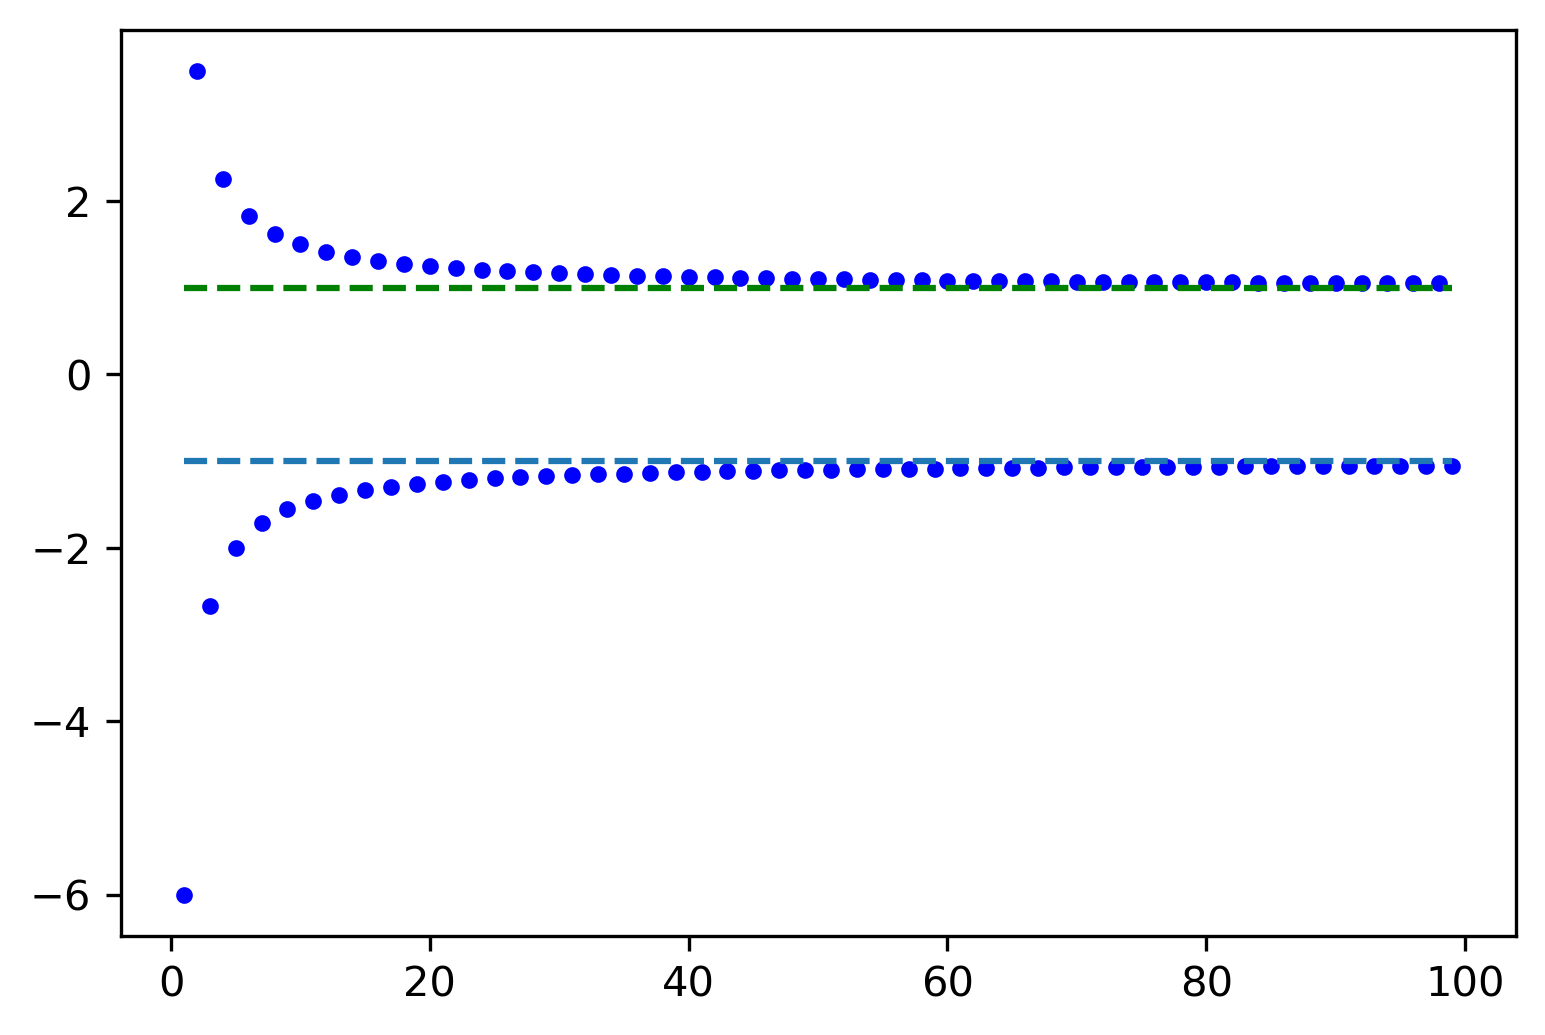
\includegraphics[height=2in,width=3in]{lim_sup_prob.png} \hspace*{\fill}  %%% \\hspace \includegraphics{imagefile} \hspace*{\fill} to align iage in center
	\caption{$(-1)^n {(n+5) \over n}$ v/s n}
\end{figure}
\begin{proof}[Solution]
	Since in the set of subsequences of $a_n$ the least element will be the $\liminf$ and the greatest term would be $\limsup$ so. Since the -ve values are less than the +ve ones and in case of $-1 - {5 \over n}$  the least value for n gives the least of all so,we can say the first negative term of each subsequence will be the element of subsequential infimimum.Therefore, $\lim (-1 - {5 \over n}) = -1$ is  the $\liminf$.
	Similar argument for $\limsup$ as the greatest of all will be sup of each subsequence and the least value of n will give the largest of all. So, the sequence $ s_n = {(n+5) \over n}$
	will be sequence of subsequential supremum.And $\lim {(n+5) \over n} = 1$.
\end{proof}


\begin{theorem}{}
	Let $(s_n)$ be a sequence $\mathbb{R}$
	\begin{enumerate}[(i)]
		\item 
		If $\lim s_n$ is defined then:
		$$\liminf s_n = \limsup s_n = \lim s_n$$
		\item
		If $\liminf s_n = \limsup s_n$ then $\lim s_n$ is defined and $\liminf s_n = \limsup s_n = \lim s_n$
	\end{enumerate}
\end{theorem}
\begin{definition}[\bf $\mathcal{CAUCHY\ SEQUENCE}$]{}\cite{wikicauchy}
	A sequence $(s_n)$ of real numbers is said to be Cauchy if:
	
	for each $\epsilon>0$ there exist a N such  :
	
	\begin{equation*}
	\forall\ n,m>N\ \mathit{implies}\ |s_n - s_m|<\epsilon
	\end{equation*}
\end{definition}
\begin{figure}[hbt!]
	
	\subfloat[The plot of a Cauchy sequence $(x_n)$, shown in blue, as $(x_n)$ versus n]
	{{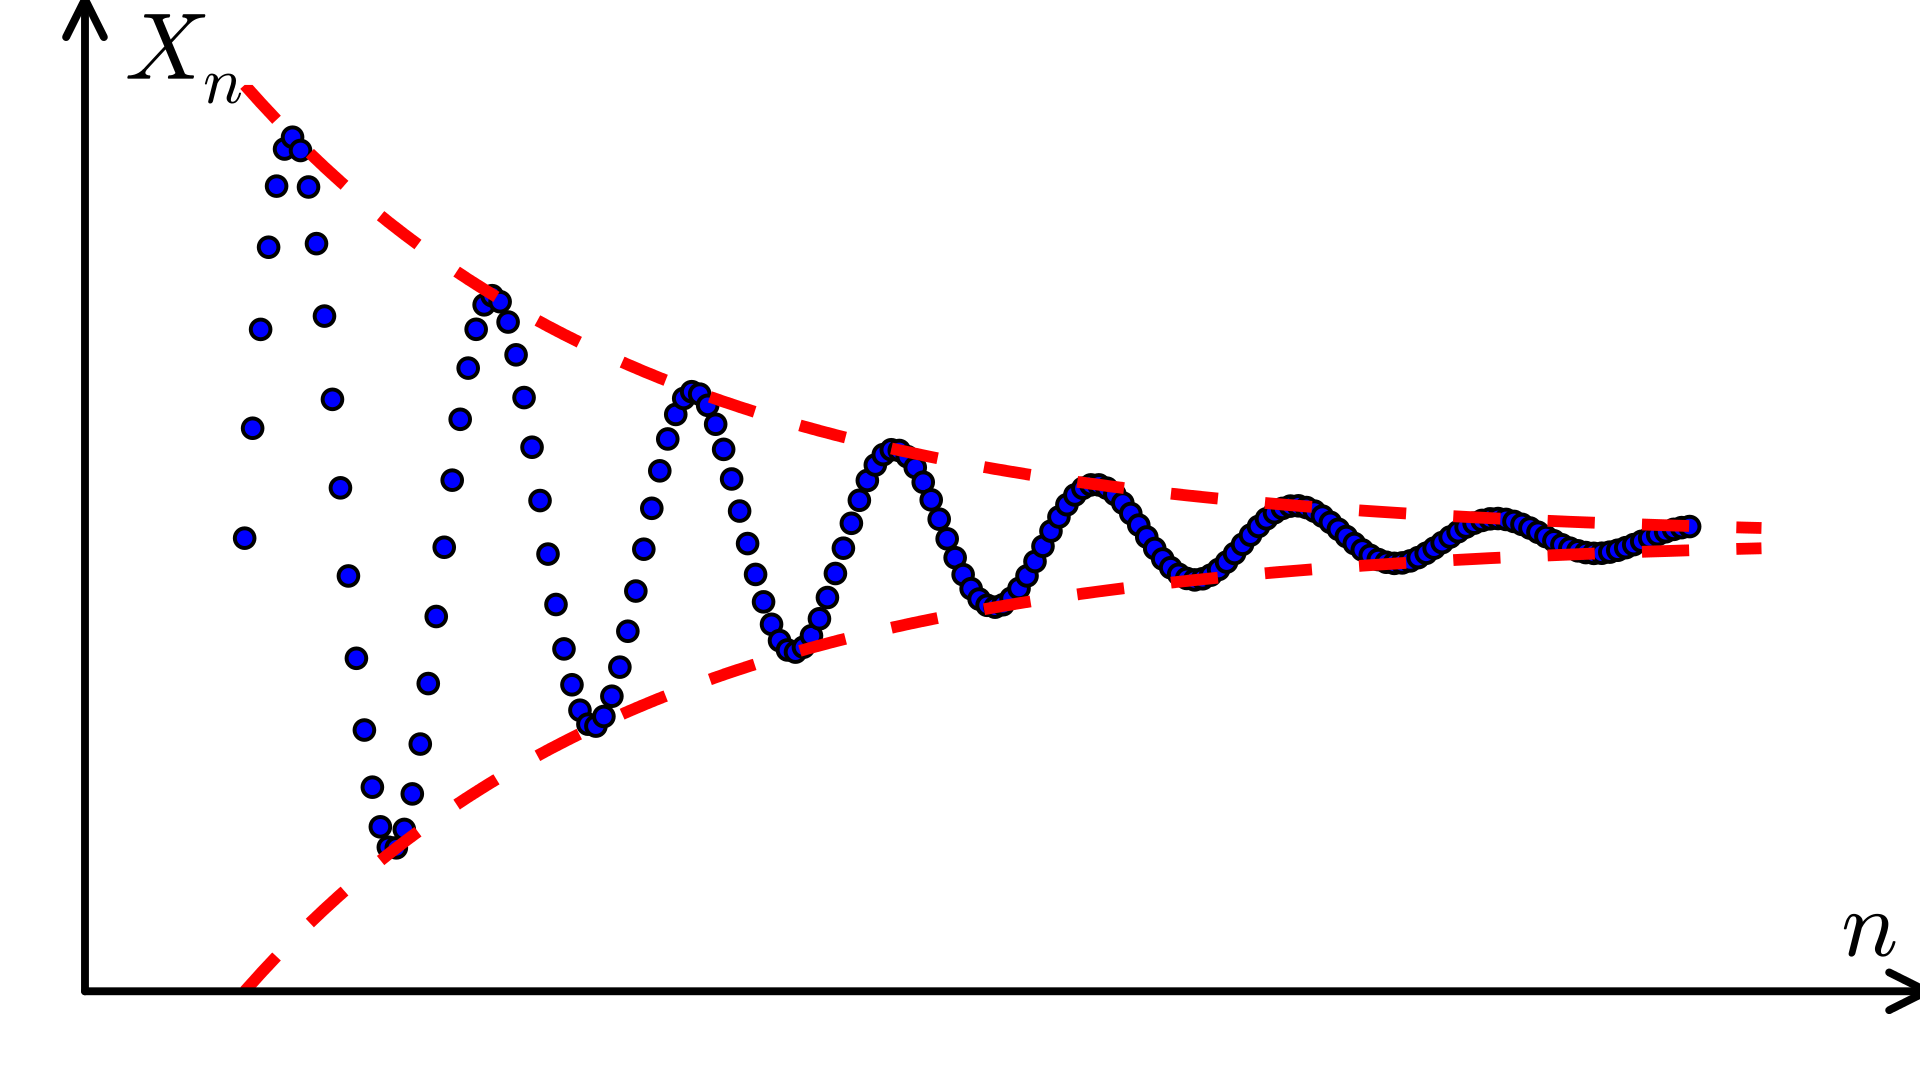
\includegraphics[width=2.5in]{cauchy_yes.png} }}%
	\qquad
	\subfloat[A sequence that is not Cauchy.But is bounded]
	{{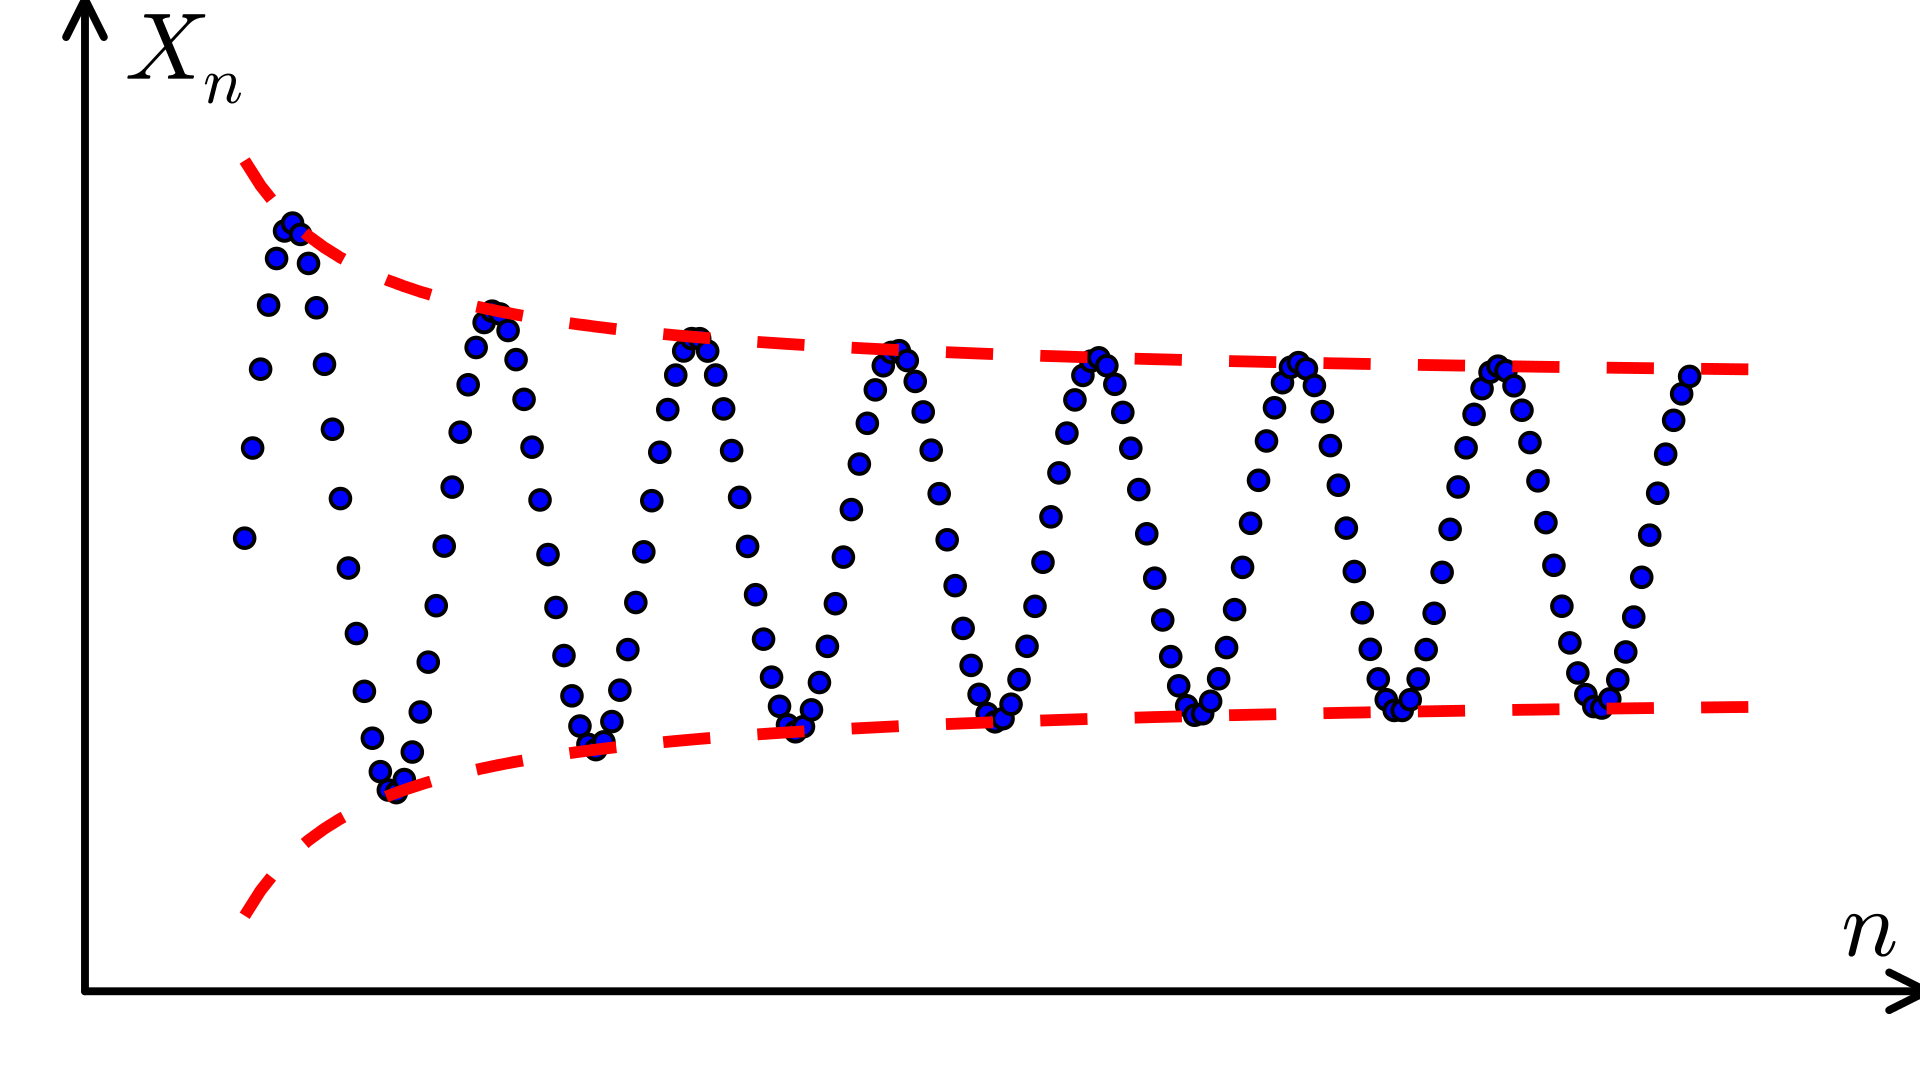
\includegraphics[width=2.5in]{cauchy_no.png} }}%
	\caption{Illustartion for cauchy sequences}%
\end{figure}
\begin{lemma}{}
	Convergent sequence are Cauchy
\end{lemma}
\begin{lemma}{}
	Cauchy sequence are bounded
\end{lemma}
\begin{theorem}{}
	A sequence is a convergent sequence if and only if it is a Cauchy
	sequence.
\end{theorem}
\paragraph{}
\begin{problem}
	Prove that $\abs{s_{n+1}-s_n} < 2^{-n}$ is cauchy. And hence convergent.
	\label{problem-2^n}
\end{problem}
\begin{proof}
	We've to prove that $\forall \epsilon>0$ there exist a N such that $\forall\ n,m>N$, $\abs{s_{m}-s_n} < \epsilon$.
	
	Take $m>n$ and let $m = n+k$. So, by triangular inequality 
	$$
	\abs{s_m - s_n} \leq \abs{s_m - s_{m-1}} + \abs{s_{m-1}+s_{m-2}}+ \ldots+ \abs{s_{n+1}+s_n} < {1 \over 2^{n}} + {1 \over 2^{n+1}} +\ldots+{1 \over 2^{m}}
	$$
	Since, m = n+k and if we add more +ve terms then we will get a G.P. with ratio $\frac{1}{2}$ which look like this:
	$$
	{1 \over 2^{n}} + {1 \over 2^{n+1}} +\ldots+{1 \over 2^{m}} = {1 \over 2^{n}} + {1 \over 2^{n+1}} +\ldots+{1 \over 2^{n+k}} = {1 \over 2^{n-1}}(1 - {1 \over 2^k})
	$$
	So,\todo[color = white,shadow]{We have not talked about Series / summation till now. Series, will be discussed in the next Section(3)} $$
	\abs{s_m - s_n} \leq \abs{s_m - s_{m-1}} + \abs{s_{m-1}+s_{m-2}}+ \ldots+ \abs{s_{n+1}+s_n}<{1 \over 2^{n-1}}(1 - {1 \over 2^k})<{1 \over 2^{n-1}}$$
	
	And applying Theorem \ref{def:basic-example} ,we can say ${1 \over 2^{n-1}}$ is convergent. Hence, the same N will work for the sequence $s_n$.
\end{proof}
\begin{problem}
	Let $s_n$ be an increasing sequence. Prove that $\sigma_n = {1 \over n}(s_1 + s_2 + \ldots+s_n)$ is an increasing sequence.
\end{problem}
\begin{proof}
	Since, since $\sigma_1 < \sigma_2$. Let us suppose $\sigma_n > \sigma_{n-1}$. Now, we have to prove that it is true for the term $\sigma_{n+1}$.
	
	Suppose, it's not true i.e. $\sigma_{n+1}<\sigma_n$  
	$$ {1 \over {n+1}}(s_1 + s_2 + \ldots + s_{n+1}) < {1 \over {n}}(s_1 + s_2 + \ldots + s_{n})$$
	If we further simplify the inequality, we get $ns_{n+1}<(s_1 + s_2 + \ldots + s_{n})$ which is false.
	So, the assumption was false. Hence, $\sigma_{n+1} > \sigma_n$.
\end{proof}
\begin{problem}
	Define $x_1 = 2$ and:
	
	$$  x_{n+1} = {1 \over 2}\left(x_n + {2 \over x_n}\right) $$
	
	Prove that the $\lim\limits_{n \to \infty} x_n = \sqrt{2}$.
\end{problem}
\begin{proof}
	Observer that $x_2 < x_1 = 2$. So, assume $x_{n+1}<x_{n}<x_{n-1}\ldots<x_1 = 2$.
	
	Suppose $x_{n+2}>x_{n+1}$ (it would lead to a contradiction), it implies:
	$$ \Rightarrow {1 \over 2}\left(x_{n+1} + {2 \over x_{n+1}}\right) > x_{n+1}$$
	$$ \Rightarrow (x_{n+1})^2<2$$
	Substitute $x_{n+1} = {1 \over 2}\left(x_n + {2 \over x_n}\right)$ and solve. We get:
	$$ ({x_{n}}^2 - 2)^2 <0$$
	which is a contradiction. So, the series is monotonically decreasing and bounded(because each element is greater than zero and less that two). Hence, convergent.
	To prove $\lim\limits_{n \to \infty} x_n = \sqrt{2}$, put $x_{n+1} = x_n = x$ in the definition.($\because \lim\limits_{n \to \infty} x_n = \lim\limits_{n \to \infty} x_{n+1}$ )
\end{proof}
\paragraph{}
\section{Subsequences}

\paragraph{An unformal definition of subsequence:}


A \textbf{Subsequence} is a sequence that can be derived from another sequence by deleting some or no elements
without changing the order of the remaining elements

\begin{theorem}{}
	If the sequence $(s_n)$ converges, then every subsequence converges to
	the same limit.
\end{theorem}

%%%%% Proof left %%%%%%%

\begin{theorem}{}
	Every sequence $(s_n)$ has a monotonic subsequence.
	
\end{theorem}
%%%%%%%%% Proof Left %%%%%%%%

\begin{theorem}[\bf Bolzano-Weierstrass Theorem]{}\cite{wikib}
	Every bounded sequence has a convergent subsequence.
	
	
	
\end{theorem}
\begin{figure}[!h]  % the command in [] to keep it under the theorem or it will be placed above the page
	\begin{center}
		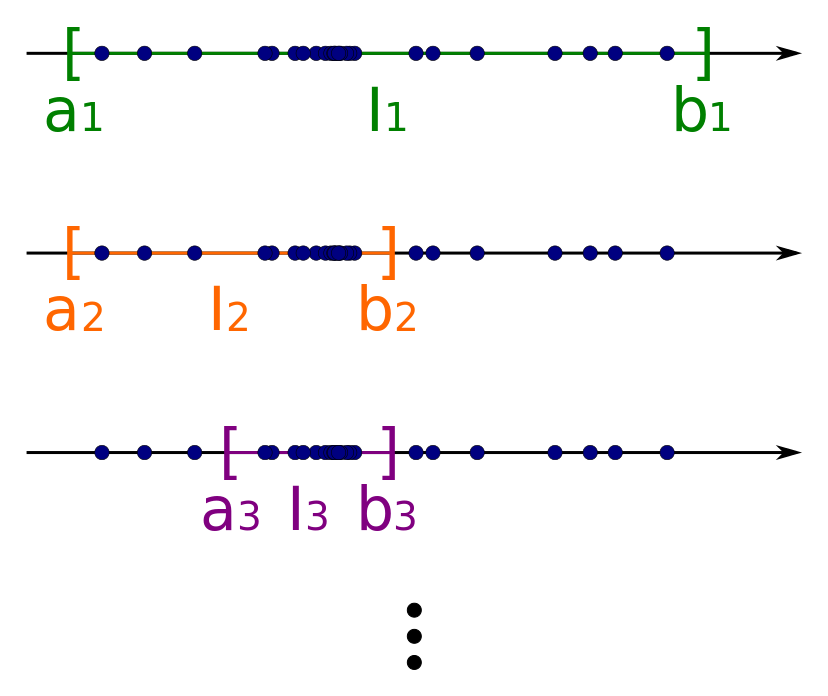
\includegraphics[width=3in]{bolanzo.png}
		\caption{Bolzano-Weierstrass Theorem}
	\end{center}
\end{figure}
\begin{proof}
	It's easy to prove that every bounded sequence has a convergent subsequence. Since, every sequence has a monotonic subsequence and since  the sequence is bounded implies subsequence is bounded. And every bounded monotonic sequence is convergent.
\end{proof}
%%%%%%%%%%%%%%%%%%%%%%%%%%%%%%%%%%%%%%%%%%%%%%%%%%%%%
\subsection{Subsequential Limits}
\begin{definition}{}
	Let $(s_n)$ be a sequence in $\mathbb{R}$. A subsequential limit is any real number
	or symbol $+\infty$ or $-\infty$ that is the limit of some subsequence of $(s_n)$.
	
	When a sequence has a limit s, then all subsequences have limit
	s, so \{s\} is the set of subsequential limits
\end{definition}
%%%%%%%%%%%%%%%%%%%%%%%%%%%%%%%%%%%%%%%%%%%%%%%%%%%%%%

%%%   Most part of subsequential limits was not covered in the class. sSo, I'll skip it 

%%%%%%%%%%%%%%%%%%%%%%%%%%%%%%%%%%%%%%%%%%%%%%%%%%%%%%
\begin{theorem}{thm:problemlim}
	Let $(s_n)$ be any sequence. There exists a monotonic subsequence
	whose limit is $\limsup s_n$, and there exists a monotonic subsequence
	whose limit is $\liminf s_n$.
\end{theorem}
\paragraph{Recall }
Let $(s_n)$ be any sequence of real numbers, and let S be the set of
subsequential limits of $(s_n)$. Recall
$$\liminf s_n  = \lim_{N\to \infty} \inf \{s_n\ :\ n>N\} = \inf S$$
and
$$\limsup s_n  = \lim_{N\to \infty} \sup \{s_n\ :\ n>N\} = \sup S$$
\paragraph{}

	\chapter{Series}
\section{Sum to infinity?}
\begin{definition}[Summation Notation]{}
	 $\sum_{n}^{m} a_k= a_n+a_{n+1}+\ldots + a_m$
	
	2.To assign meaning to $\sum_{n=m}^{\infty} a_n$, we consider the sequences $(s_n)_{n=m}^{\infty}$
	of partial sums:
	$$s_n = a_m + a_{m+1} + \ldots + a_n = \sum_{k=m}^{n} a_k$$
	The infinite series $\sum_{n=m}^{\infty} a_n$ an is said to converge provided the sequence
	$(s_n)$ of partial sums converges to a real number S, in which case we
	define $$\sum_{n=m}^{\infty} a_n =  S$$
\end{definition}


\begin{definition}[Cauchy Criterion for Series Convergence]{}
	We say a series $\sum a_n$ satisfies the Cauchy criterion if its sequence
	$(s_n)$ of partial sums is a Cauchy sequence i.e.:
	
	
	for each $\epsilon > 0$ there exists a number N such that:
	
	$$n \geq m>N\ \text{implies}\ \abs{s_n - s_{m-1} }<\epsilon$$
	And, $s_n - s_{m-1} = \sum_{n}^{m} a_k$
	
	
	A series converges iff it satisfies cauchy criterion
\end{definition}
\begin{corollary}{cor:lim0}
	If $\sum a_n$ converges then $\lim a_n = 0$
\end{corollary}
%%%%%%%%%%%%%%%%%%%%%
%% I'm leaving most of the part from the book

%%%%%%%%%%%%%%%%%%%%%
\section{Convergence Tests for Series}
\paragraph{\S Comparison Test}
Let $\sum a_n$ be a series where $a_n \geq  0$  for all n.
\begin{enumerate}
	\item
	If $\sum a_n$ converges and $|b_n|\leq a_n $ for all n, then $\sum b_n$ converges.
	\item
	If $\sum a_n = + \infty$ and $b_n \geq a_n$ for all n, then $\sum b_n = + \infty$
\end{enumerate}
\begin{problem}
	Show that the series $s_n = \sum {1 \over n^2}$ converges
	\label{1 by n^2}
\end{problem}
\begin{proof}[Solution]
	Observation:$$
	\Rightarrow {1 \over n^2}  < {1 \over n(n-1)} = {1 \over n-1} - {1 \over n}
	$$
	$$
	\Rightarrow \sum_{2}^{n} {1 \over n^2} < \sum_{2}^{n}	\left({1 \over n-1} - {1 \over n}\right)
	$$
	Or  
	$$
	\Rightarrow 1+\sum_{2}^{n} {1 \over n^2} < 1+\sum_{2}^{n}	\left({1 \over n-1} - {1 \over n}\right)
	$$
	$$
	\Rightarrow \sum_{2}^{n} {1 \over n^2} <2 - \frac{1}{n}
	$$
	As $n \to \infty$ we get:
	$$\sum_{2}^{\infty} {1 \over n^2} < 2 $$
	Hence, it converges.
\end{proof}

\paragraph{\S\ Ratio Test:}\cite{wikiratio}
A series $\sum a_n$ of nonzero terms.The usual form of the test makes use of the limit:
$$L =  \lim_{n \to \infty} \abs{a_{n+1 } \over a_n}$$
\begin{enumerate}[\bf (i)]
	\item
	if $L < 1$ then the series converges absolutely;
	\item
	if $L > 1$ then the series diverges;
	\item
	if $L = 1$ or the limit fails to exist, then the test is inconclusive, because there exist both convergent and divergent series that satisfy this case.
\end{enumerate}
It is possible to make the ratio test applicable to certain cases where the limit L fails to exist, if limit superior and limit inferior are used. The test criteria can also be refined so that the test is sometimes conclusive even when L = 1. More specifically, let
\begin{itemize}
	\item
	$ R = \limsup \abs{a_{n+1 } \over a_n}$
	\item  $ r = \liminf \abs{a_{n+1 } \over a_n}$
\end{itemize}
Then the ratio test states that:
\begin{itemize}
	\item if $R < 1$, the series converges absolutely;
	\item if $r > 1$, the series diverges;
	\item if $\abs{a_{n+1 } \over a_n} \geq 1$ for all large n (regardless of the value of r), the series also diverges; this is because $|a_{n}|$ is nonzero and increasing and hence an does not approach zero;
	\item the test is otherwise inconclusive
\end{itemize}
\paragraph{\S\ Root Test:}\cite{wikiroot}
Let $\sum a_n$ be a series and let $ \alpha = \limsup |a_n|^{1/n}$. The series $\sum a_n$

\begin{enumerate}[\bf (i)]
	\item
	converges absolutely if $\alpha<1$.
	\item
	diverges if $\alpha>1$.
	\item
	Otherwise $\alpha = 1$ and the test gives no information
\end{enumerate}
Note that if:
$$ \lim\limits_{n \to \infty} \sqrt[n]{|a_n|}$$
converges then it equals $\alpha$ and may be used in the root test instead.
\begin{lemma}{}
	Let $|s_n|$ be a sequence of non-zero real numbers,\par
	Then, $$\liminf \abs{\frac{s_{n+1}}{s_n}} \leq \liminf\abs{|s_n|^{1 \over n}} \leq \limsup\abs{|s_n|^{1 \over n}} \leq \limsup \abs{\frac{s_{n+1}}{s_n}}$$
	
\end{lemma}
\paragraph{}
\begin{problem}
	Prove that $ \lim_{n \to \infty} {x^n \over n!} = 0$
\end{problem}

\begin{proof}[\bf Solution]
	
	\begin{enumerate}[a.]
		\item
		Given: 
		\begin{gather*}
		\Rightarrow	a_n = {x^n \over n!} \\
		\Rightarrow 	a_{n+1} = {x^{n+1} \over {n+1}!} \\
		\Rightarrow	{a_{n+1} \over a_n} = {x \over {n+1}}
		\end{gather*}
		As $ n \to \infty$ ratio ${a_{n+1} \over a_n} \to 0$. Thus it converges\textsuperscript{\href{https://math.stackexchange.com/q/712586}{1 }}. That means the series $\sum {x^n \over n!}$ converges therefore ${x^n \over n!}$ converges to zero. 
		
		\item
		The series $e^x = \sum_{n=0}^{\infty} {x^n \over n!}$ converges.
		Hence ${x^n \over n!} \to 0$.
		\item
		\href{https://math.stackexchange.com/questions/712572/prove-that-xn-n-converges-to-0-for-all-x}{MathStackexchange}
	\end{enumerate}
\end{proof}
\begin{problem}
Let $\limsup |a_n| > 0$. Then prove that $\limsup |a_n| ^ {1 \over n} \geq 1$.
\end{problem}
\begin{proof}
	Assume that $\limsup |a_n| > 0$ but $\limsup |a_n| ^ {1 \over n} < 1$.  We also conclude that $\limsup |a_n| ^ {1 \over n} < 1 $ implies $\sum a_n $ converges absolutely (by Root test).So, $\lim |a_n|=\limsup |a_n| = 0$. Contradiction!. So, $\limsup |a_n| ^ {1 \over n} \geq 1$.
\end{proof}
\begin{theorem}{}
	Let $\sum |a_n|$ be a convergent series \& let $(b_n)$ be a bounded sequence.
	Then, $\sum a_n b_n$ is also convergent.
\end{theorem}
\begin{proof}
	By triangular inequality we can show that:
	$$ \left|\sum_{k = m}^{n} a_k b_k  \right|\leq \sum_{k = m}^{n}\abs{a_k b_k}$$
	
	Given, $|b_n| \leq M$ (it's bounded), implies:
	$$ \Rightarrow \abs{a_k}\abs{b_k} \leq \abs{a_k }M$$
	$$ \Rightarrow \sum \abs{a_k}\abs{b_k} \leq \sum \abs{a_k }M$$
	Since, $\sum a_n$ converges; therefore by cauchy criterion $\exists\ N \in \mathbb{N}$ such that $\forall\ n\geq m>N$:
	
	$$\Rightarrow \sum_{k = m}^{n} |a_k| < {\epsilon \over M}$$
	$$\Rightarrow \sum_{k = m}^{n} M|a_k| < \epsilon$$
	Or
	$$\Rightarrow\left|\sum_{k = m}^{n} a_k b_k  \right|\leq \sum \abs{a_k}\abs{b_k} \leq \sum_{k = m}^{n} M|a_k| < \epsilon$$
	Hence, $\sum a_n b_n$ is convergent by comparison test.
\end{proof}
\begin{corollary}{}
	Let $ a_n \geq 0$ \& $\sum a_n$ converges. 
	Then
	$ \sum (a_k) ^ p$ converges $\forall\ p>1$ 
\end{corollary}
\begin{proof}The above expression can be rewritten as:
	$$  \sum_{k=m}^{n} \abs{a_k}^p = \sum_{k=m}^{n} \abs{a_k}\abs{a_k}^{p-1}$$
	
	Since,  $\sum a_n$ converges, therefore $a_n \to 0$. So, sequence $a_n$ is convergent, hence bounded.So, $a_k ^{p-1}$ is bounded.
	
	$\therefore$ By previous theorem, we can say
	$ \sum (a_k) ^ p$ converges.
\end{proof}
\section{Alternating Series Test}
\begin{theorem}{}
	If $a_1 \geq a_2 \geq \ldots \geq a_n \geq \ldots \geq 0$ and $\lim a_n = 0$, then the alternating series $\sum (- 1)^{n+1}a_n$ converges. Moreover, the partial sums $s_n =\sum_{k = 1}^{n} ( - 1)^{k+1}a_k$ satisfy $|s - s_n|\leq a_n$ for all n.
\end{theorem}
\begin{proof}
	We need to show that the sequence $(s_n)$ converges. Note that the
	subsequence $(s_{2n})$ is increasing because $s_{2n+2} - s_{2n} =  - a_{2n+2} +
	a_{2n+1}\geq  0$. Similarly, the subsequence $(s_{2n - 1})$ is decreasing since
	$s_{2n+1} - s_{2n - 1} = a_{2n+1} - a_{2n}\leq 0$. We claim:
	
	$$      s_{2m} \leq s_{2n+1}\quad \text{for all }\quad m,n \in \mathbb{N}           $$
	First note that $s_{2n} \leq s_{2n+1}$ for all n, because $s_{2n+1} - s_{2n} = a_{2n+1} \geq 0$.
	If $m\leq  n$, then the above equation holds because $s_{2m} \leq s_{2n} \leq s_{2n+1}$. If $m \geq n$,
	then equation  holds because $s_{2n+1}\geq s_{2m+1 }\geq  s_{2m}$.  We
	see that $(s_{2n}) $ is an increasing subsequence of $(s_n)$ bounded above
	by each odd partial sum, and $(s_{2n+1})$ is a decreasing subsequence
	of $(s_n)$ bounded below by each even partial sum. By Theorem (\ref{bounded}),
	these subsequences converge, say to s and t. Now 
	$$ t - s = \lim_{n \to \infty} s_{2n+1} - \lim_{n \to \infty}s_{2n} = \lim\limits_{n \to \infty}(s_{2n+1} - s_{2n}) = \lim\limits_{n \to \infty}a_{2n+1} = 0$$
	. so s = t, follows that $\lim_{n}s_n = s$.
	
	To check the last claim, note that $s_{2k} \leq s \leq s_{2k+1}$, so both
	$s_{2k+1} - s$ and $s - s_{2k}$ are clearly bounded by $s_{2k+1} - s_{2k} = a_{2k+1} \leq a_{2k}$.
	So, whether n is even or odd, we have $|s - s_n| \leq a_n$.
\end{proof}
\section{Integral Test}

\begin{theorem}{}
	Consider an integer N and a non-negative function $f$ defined on the unbounded interval $ [N,\infty) $, on which it is monotone decreasing. Then the infinite series:
	$$ \sum_{n}^{\infty} f(n)$$
	converges to a real number if and only if the improper integral
	
	$$ \int_{N}^{\infty} f(x)dx$$
	is finite. In other words, if the integral diverges, then the series diverges as well.
\end{theorem}


\paragraph{}
\begin{problem}
	Let $(a_n)_{n \in \mathbb{N}}$  be a sequence such that $\liminf |a_n| = 0$. Prove there is
	a subsequence $ (a_{n_k})_{k \in \mathbb{N}} $ such that $\sum_{k = 1}^{\infty}(a_{n_k})$ converges.
\end{problem}
\begin{proof}
	We first set $n_0=1$ and $c_1=1$. By the property of $\liminf$, there exists $n_1>n_0=1$ such that $|a_{n_1}|<c_1=1$. Why does such an $n_1$ exist? For sake of contradiction, assume there is no $n \in \mathbb{N}$ such that $|a_n| < 1$, then 1 would be a lower
	bound for $\{a_n : n \in \mathbb{N}\}$. In which case, for all N, 1 would be a
	lower bound for $\{a_n : n > \mathbb{N}\}$ so that $1\leq  inf \{a_n : n > \mathbb{N}\}$, in
	which case $1 \leq \lim_{N\to\infty} \inf \{a_n : n > \mathbb{N}\}$, so we would get $1 \leq0$. A contradiction.
	
	Then we set $c_2=1/4$. Again, there exists $n_2>n_1$ such that $|a_{n_2}|<c_2=1/4$. Why does such an $n_2$ exist? (the same argument can be used here as above)
	
	We can continue this fashion. At the $k$-th step, we set $c_k=1/k^2$ and we can then find some $n_k>n_{k-1}$ such that $|a_{n_k}|<c_k=1/k^2$. 
	
	Note that 
	$$\sum_{k=1}^\infty{|a_{n_k}|}<\sum_{k=1}^\infty{\frac{1}{k^2}}.$$
	
	Since the RHS converges, the LHS converges, i.e., $\sum_{k=1}^\infty{a_{n_k}}$ converges absolutely. 
\end{proof}
\begin{problem}
	Prove if $(a_n)$ is a decreasing sequence of real numbers and if $\sum a_n$
	converges, then $\lim n\cdot a_n = 0$.
\end{problem}
\begin{proof}
	Since it's given that $\sum a_n$ converges. Therefore by cauchy criteria $\forall \epsilon>0$ $\exists N \in \mathbb{N}$ such that $\forall n> m+1>N$: (we'll be using the fact that for $n>m$ we have $a_n<a_m$)
	$$ \sum_{m+1}^{n} a_k <\epsilon    $$ \todo[color = white]{we didn't use a mod because observe that all terms are positive}	
	
	$$ (n-m)a_n \leq  a_{m+1}+a_{m+2} \cdots +a_n   <\epsilon$$
	
	Hence, $\lim_{n \to \infty} (n-m)a_n = 0$. Further, we see that :
	$$ \lim\limits_{n \to \infty} n a_n = \lim_{n \to \infty} (n-m)a_n + \lim_{n \to \infty} m a_n   = 0$$
\end{proof}
\begin{problem}
	Show that $\sum {1 \over n^p}$ converges iff $p > 1$
\end{problem}
\begin{proof}
	\begin{enumerate}
		\item
		In particular, for $p\leq 1$, we can write $\sum{1 \over n^p}  = + \infty$.
		For $ p = 2$ we have already proved it in Problem \ref{1 by n^2}.
		
		For $p>2$, we can prove it by the comparison test as :
		
		$$ \left\{{1 \over n^p } < {1 \over n^2}\right\}, \quad \forall \quad p>0$$ 
		Since, ${1 \over n^2}$ converges. Then ${1 \over n^p}$ converges by comparison test.
		\begin{center}
			Or
		\end{center}
		The above proposition can be used to prove the result for $p>2$
		
		\item
		\begin{figure}[h!]  % the command in [] to keep it under the theorem or it will be placed above the page
			\begin{center}
				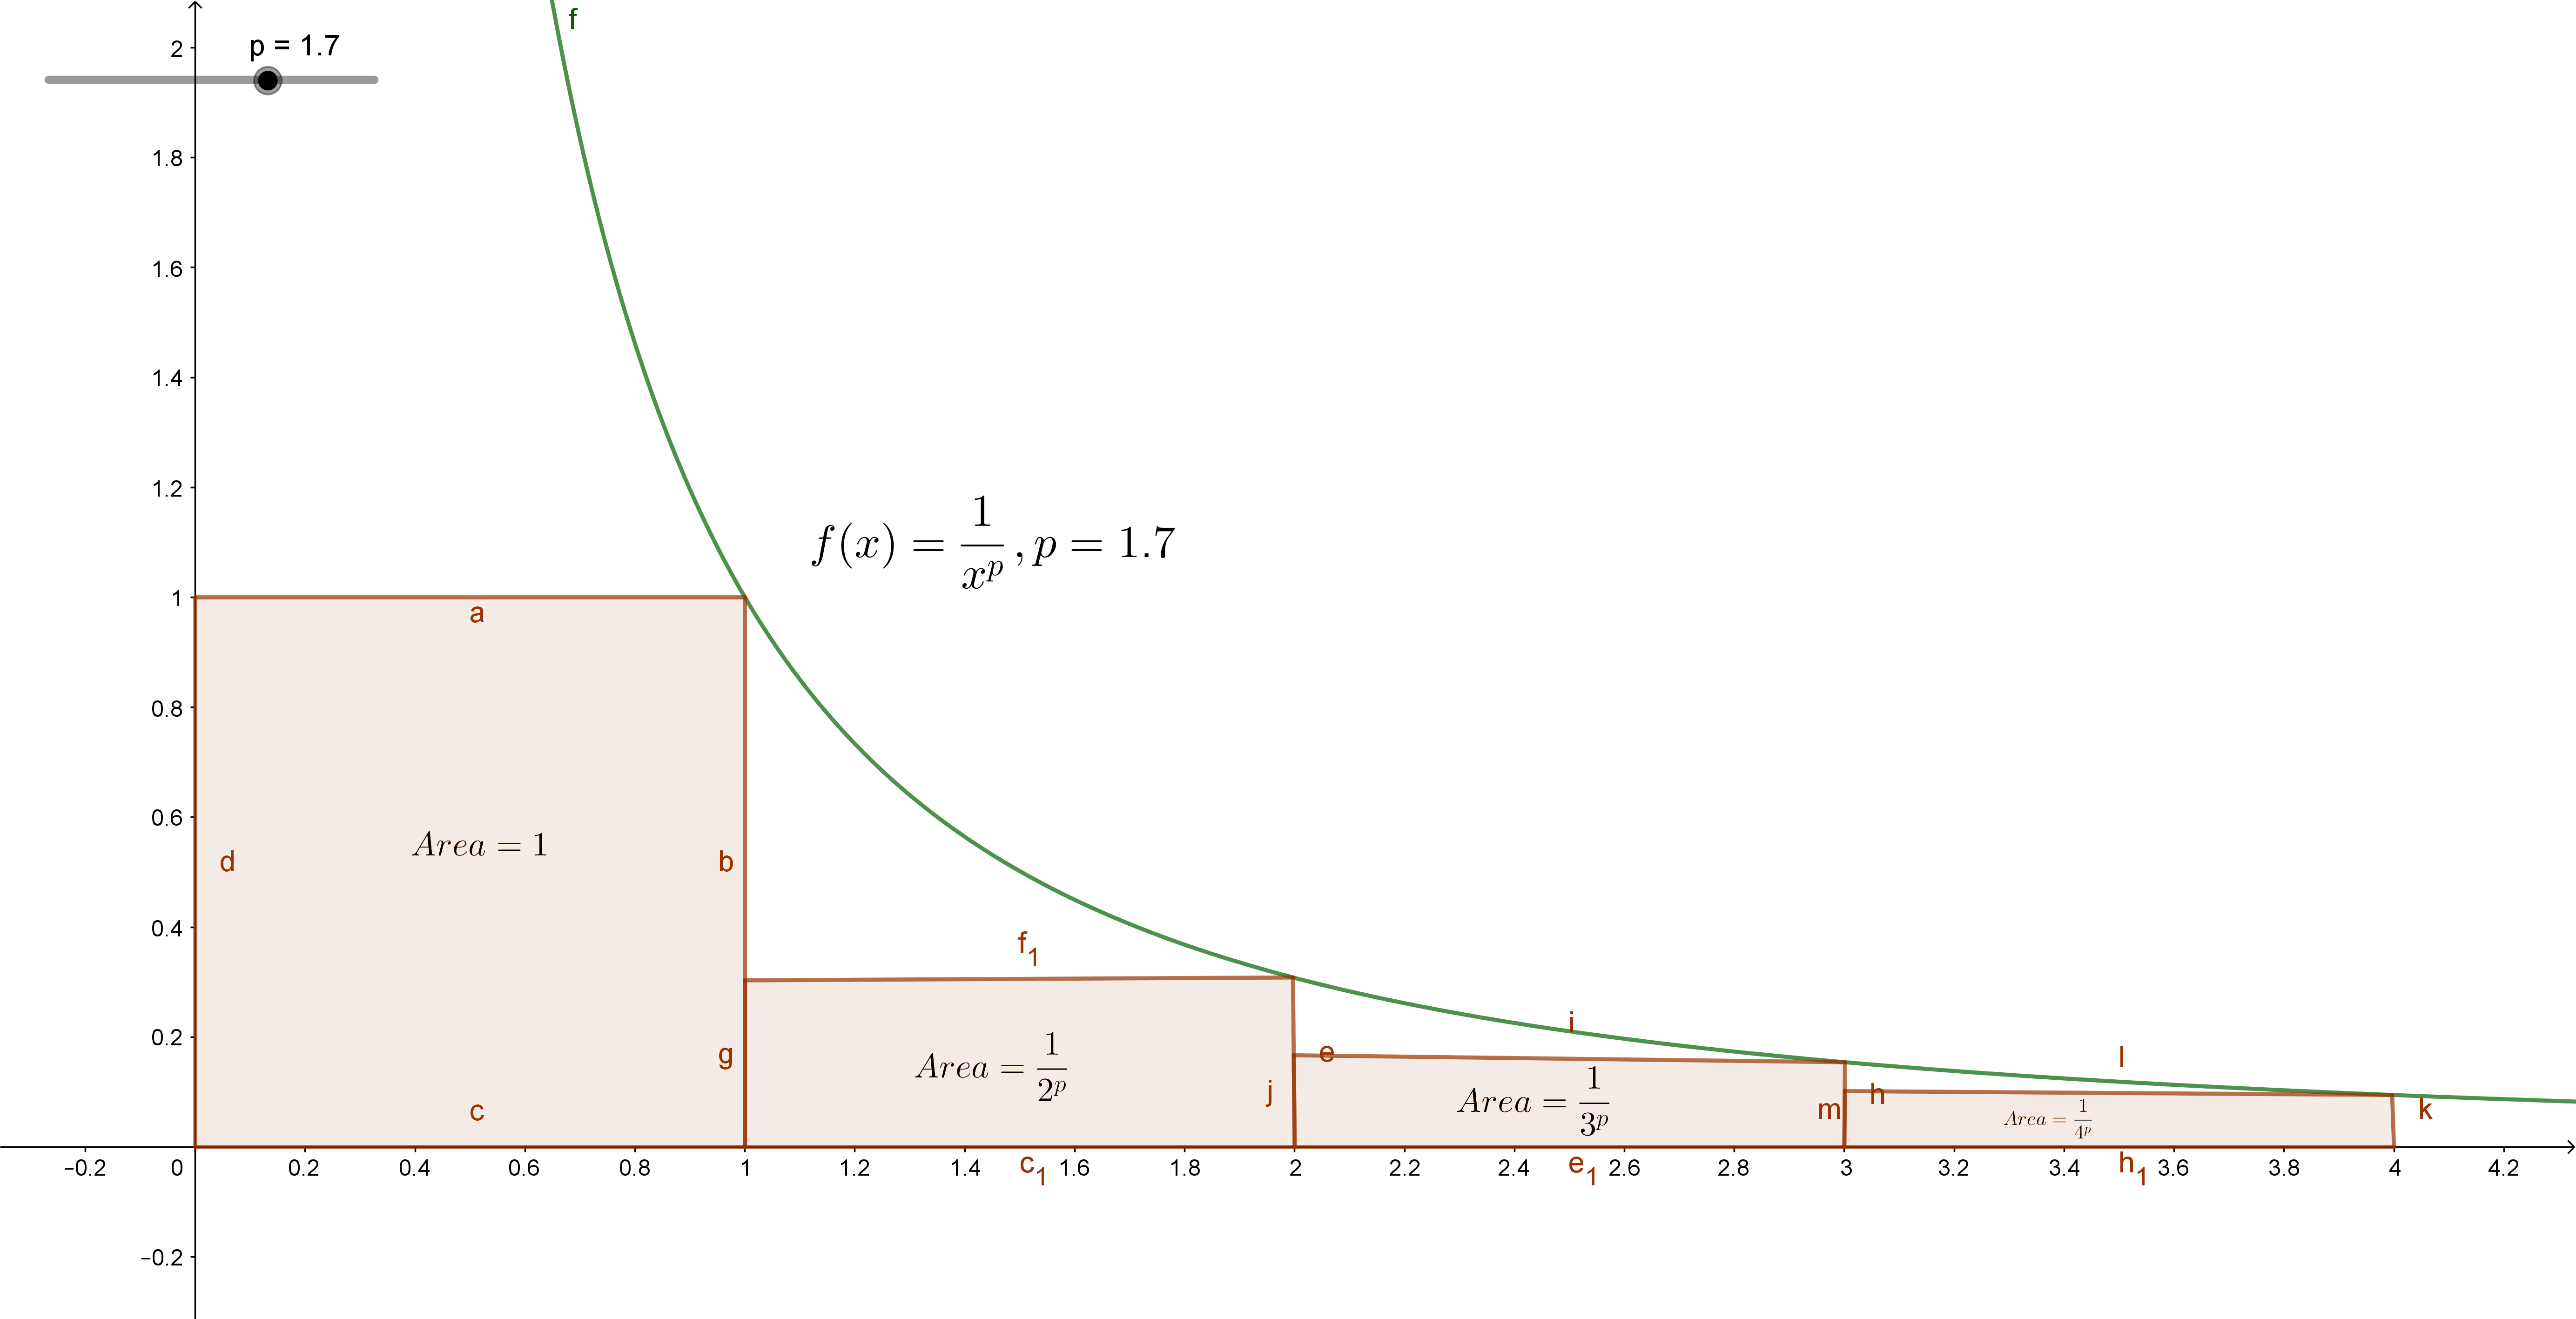
\includegraphics[width=\textwidth]{geogebra.png}
				\caption{Geometric intution for $\sum{1 \over n^p }$}
			\end{center}
		\end{figure}
		For $ 1 < p<2$
		
		We have,
		$$ \underbrace{\sum_{k=1}^{n} {1 \over k^p}}_{\substack{ \text{sum of rectangles going} \\ \text{from 1 $\to$ n}}} \leq \underbrace{1 + \int_{1}^{n} {1 \over x^p}dx}_\text{area under the curve} $$
		$$   \Rightarrow \sum_{k=1}^{n} {1 \over k^p} \leq 1 + \left[ x^{1-p} \over {1-p} \right]_{1}^{n}      $$
		$$ \Rightarrow   \sum_{k=1}^{n} {1 \over k^p} \leq 1 + \left[ {n^{1-p} \over {1-p} } - {1 \over {1-p}}\right]     $$
		$$ \Rightarrow   \sum_{k=1}^{n} {1 \over k^p} \leq \left[ {p - n^{1-p} \over p-1} \right]     $$
		
		As $ n\to \infty$ we get( $\because$ $1-p<0$),
		$$ \Rightarrow   \sum_{k=1}^{n} {1 \over k^p} \leq \left[ {p \over p-1} \right]     $$
	
	\end{enumerate}
	
\end{proof}

\chapter{Continuity}

\section{Continuity and Functions}
\paragraph{}
\begin{definition}{}
	A function $f$ whose domain is defined over $\mathbb{R}$ is said to be continuous at a point
	$x_0\in dom(f)$ iff:
	
	for each $\epsilon>0$ there exist a $\delta>0$ such that:
	$$x\in dom(f)\ \textit{and}\ \abs{x-x_0}<\delta\ \textit{imply}\ \abs{f(x)-f(x_0)}<\epsilon$$.
	
	
	
	\begin{center}
		\textbf{Or}
	\end{center}
	
	Let $f$ be a real-valued function whose domain is a subset of $\mathbb{R}$. The
	function $f$ is continuous at $(x_0)\in dom(f)$ if, for every sequence $(x_n)\in dom(f)$ converging to $x_0$, we have $lim_{n} f(x_n) = f(x_0)$ i.e.:
	
	if for every sequence in    domain if  $x_n\to x_0$ we have $f(x_n)\to f(x_0)$
	
\end{definition}

\begin{theorem}{}
	Let $f$ be a real-valued function with $dom(f) \subseteq \mathbb{R}$. If $f$ is continuous
	at $x_0$ in $dom(f)$, then $|f|$ and $kf$, $k \in \mathbb{R}$, are continuous at $x_0$
	
\end{theorem}
\subsection{Properties of Continuous Functions}

\paragraph{\S\ Bounded Function}
A real-valued function $f$ is said to be bounded if $\{f(x) \colon x \in dom(f)\}$
is a bounded set, i.e., if there exists a real number M such that
$|f(x)| \leq M$ for all $x \in dom(f)$.

\begin{theorem}{}
	Let $f$ be a continuous real-valued function on a closed interval $[a, b]$.
	Then $f$ is a bounded function. Moreover, $f$ assumes its maximum
	and minimum values on $[a, b]$; that is, there exist $ x_0, y_0\ \in \ [a, b]$ such
	that $f(x_0) \leq f(x) \leq f(y_0)$ for all $x \in [a, b]$.
\end{theorem}

\begin{theorem}[\bf Intermediate value theorem]{}
	If $f$ is a continuous real-valued function on an interval I, then $f$ has
	the intermediate value property on I: Whenever $a, b \in I$, $a<b$ and y
	lies between $f(a)\ \text{and}\ f(b)$ i.e. $[f(a) < y <f(b)\ or\  f(b) <y<f(a)]$,
	there exists at least one $x \in (a, b)$ such that $f(x) = y$.
	
	
\end{theorem}
\begin{figure}[h!]  % the command in [] to keep it under the theorem or it will be placed above the page
	\begin{center}
		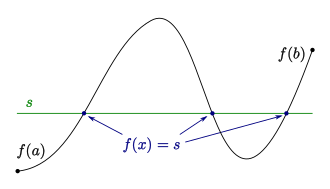
\includegraphics[]{intermediate.png}
		\caption{Intermediate value theorem}
	\end{center}
\end{figure}
\paragraph{}
\begin{problem}
	Prove that $\lim_{x \to a} \abs{x+2} = \abs{a+2}$
\end{problem}
\begin{proof}
	Simply take, $ \delta = \epsilon$. We have $ \abs{x - a} < \delta$.
	$$ 
	\abs{\abs{x+2}-\abs{a+2}} \leq \abs{x - a}     < \delta  = \epsilon \quad \text{(By triangular inequality)}$$
\end{proof}

\begin{problem}
	Prove that $\lim_{x \to a} (4+x-3x^2) = (4+a-3a^2)$
\end{problem}
\begin{proof}
	We need to prove that 
	$$ \abs{4+x-3x^2 - (4+a-3a^2)} = \abs{(x-a)-3(x-a)(x+a)} < \epsilon$$
	\begin{center}
		\textbf{Or}
	\end{center}
	$$|x - a|\abs{1-3(x+a)} < \epsilon$$
	Since, we are trying to find a $\delta$ we can apply the triangular inequality on the above expression and we get.
	
	$$|x - a|\abs{1-3(x+a)} \leq| x - a|(1+3\abs{x+a}) <\epsilon$$
	We need to find a upper bound for the above expression   $(|1+3\abs{(x+a)})$   which is not dependet on x.
	
	If we choose  $ |x - a|< \delta < {\epsilon \over |1+3 | x+a ||}$ then it would imply $|x - a|\abs{1+3(x+a)} < \epsilon$. But when we have one $\delta > 0 $ that works, any smaller value will also work. By choosing $ \delta < 1$ we would have:
	
	$$ |x - a| < 1\ \text{ when ever } \ |x - a| < \delta$$
	
	$$\Rightarrow ||x| - |a|| \leq |x - a| < 1$$ 
	Or
	$$\Rightarrow |x| < 1 + |a|$$
	$$\Rightarrow |x + a| \leq  |x| + |a| < |2a| + 1$$
	$$ \Rightarrow [1 + 3 |x+a |\ ] < [1 + 3 (1+2|a  |)\ ]$$
	
	Since, we need both the above assumptions i.e. $ | x- a| < \delta$ \& $| x- a| < 1$ to be satisfied.So,       take :
	
	$$ \delta = \min \left( 1, { \epsilon \over 1 + 3(1 + 2 | a| )}   \right)   $$
	And, whole discussion above proves that it would work.
	
\end{proof}
\begin{problem}
	Is $ \lim {{4x+1} \over 3x-4} $ is continuous for $x \not = 4/3$?
\end{problem}

%\begin{proof}
%We will break the interval in two sets 
%$ |x| > 4/3$ and $ |x|<4/3$.

%\begin{enumerate}[\bf 1.]
%\item
%Case 1: $|x|>4/3$ . $ \abs{{{4x+1} \over 3x-4} - {{4a+1} \over 3a-4}} = \frac{|x-a|19}{|3a - 4||3x-4|} $
%$$ \Rightarrow |x-a| < \frac{\epsilon |3a - 4||3x-4|}{19}$$

%We need to find a lower bound for $|x|$, so that we can find $\delta$ such that $|x-a| < \delta \leq \frac{\epsilon |3a - 4||3x-4|}{19}$. To do so, we have assumed $|x|>4/3$ implies $3|x| - 4>0$.So, using the same argument in above pooof, we can say $ ||x| - |a|| \leq |x-a| < \delta = 1$




%\item
%\end{enumerate}


%\end{proof}
\begin{problem}
	Let f and g be continuous functions on $[a, b]$ such that $f(a) \geq
	g(a)$ and $f(b) \leq g(b)$. Prove $f(x_0) = g(x_0)$ for at least one $x_0$ in
	$[a, b]$
\end{problem}
\begin{proof}
	Define $h(x) = f(x)-g(x)$. It's given that $f(a) - g(a)\geq 0$ and $f(b) - g(b)\leq 0$. So, by intermediate value theorem there exists a $x_0 \in [a,b]$. Such that $h(x_0) = 0$.
	
\end{proof}
\begin{problem}
	Suppose f is continuous on $[0, 2]$ and $f(0) = f(2)$. Prove there exist
	$x, y \in [0, 2]$ such that $|y - x| = 1$ and $f(x) = f(y)$.
\end{problem}
\begin{proof}
	Define $g(x) = f(x+1) - f(x)$ . Let $|x-y| = 1$ implies either $x = y+1$ or $y = x+1$. 
	Take anyone of them, it won't matter as we can exchange y with x for another case. 
	
	Also, $ g(0) = f(1)-f(0)$ and $g(1) = f(2)-f(1)$. Adding both the equations $g(0)+g(1) = 0$, which implies that one of them is negative of other i.e. if any one of the value is + ve  the other is - ve.
	So, there exists a value of $x \in [0,1]$ such that $g(x) = 0$ or $f(x+1) = f(x) \equiv f(y) = f(x)$.
\end{proof}
\section{Uniform Continuity}

\begin{definition}[Uniform Continuity]{}
	Let	$f$ be a real-valued function defined on a set $S \subseteq \mathbb{R}$. Then f is
	uniformly continuous on S if
	for each $\epsilon> 0$ there exists $\delta > 0$ such that
	$$ x,y \in S \ \text{and} \ \abs{x - y} < \delta \ \text{imply} \ \abs{f(x) - f(y)} < \epsilon $$
	We will say f is uniformly continuous if f is uniformly continuous
	on dom(f).
	
\end{definition}
\begin{figure}[h!]
	\centering
	\subfloat[For uniformly continuous functions, there is for each $\epsilon >0$ a $\delta >0$ such that when we draw a rectangle around each point of the graph with width  $2\delta$ and height $2\epsilon$, the graph lies completely inside the rectangle.]
	{{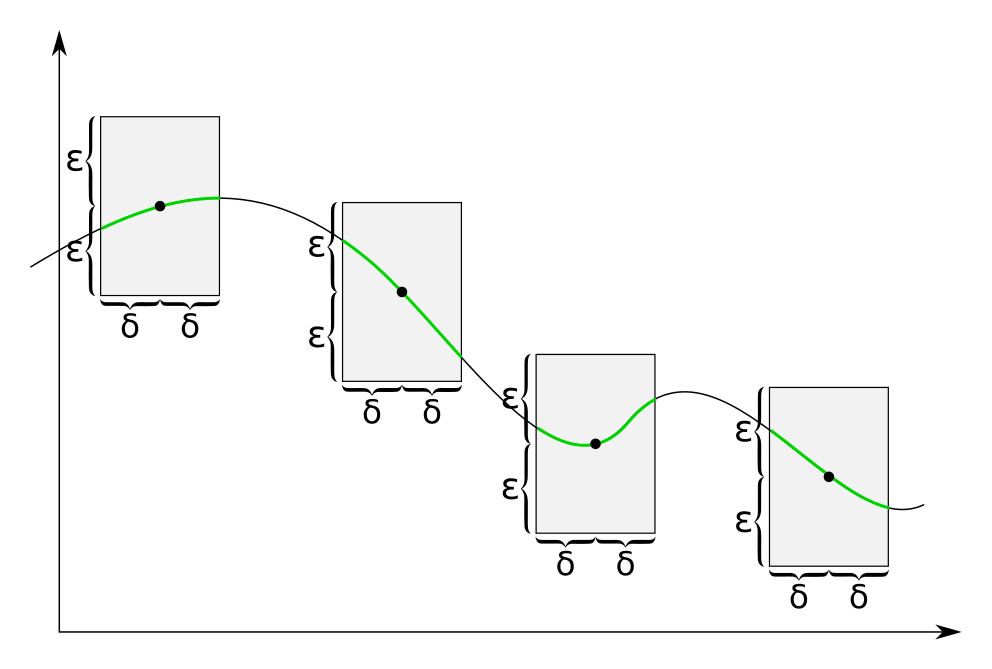
\includegraphics[width= 2.5in]{uniform_yes.png} }}%
	\qquad
	\subfloat[For functions that are not uniformly continuous, there is an $\epsilon>0$ such that regardless of the $\delta>0$ here are always points on the graph, when we draw a $2\epsilon-2\delta$ rectangle around it, there are values directly above or below the rectangle.]
	{{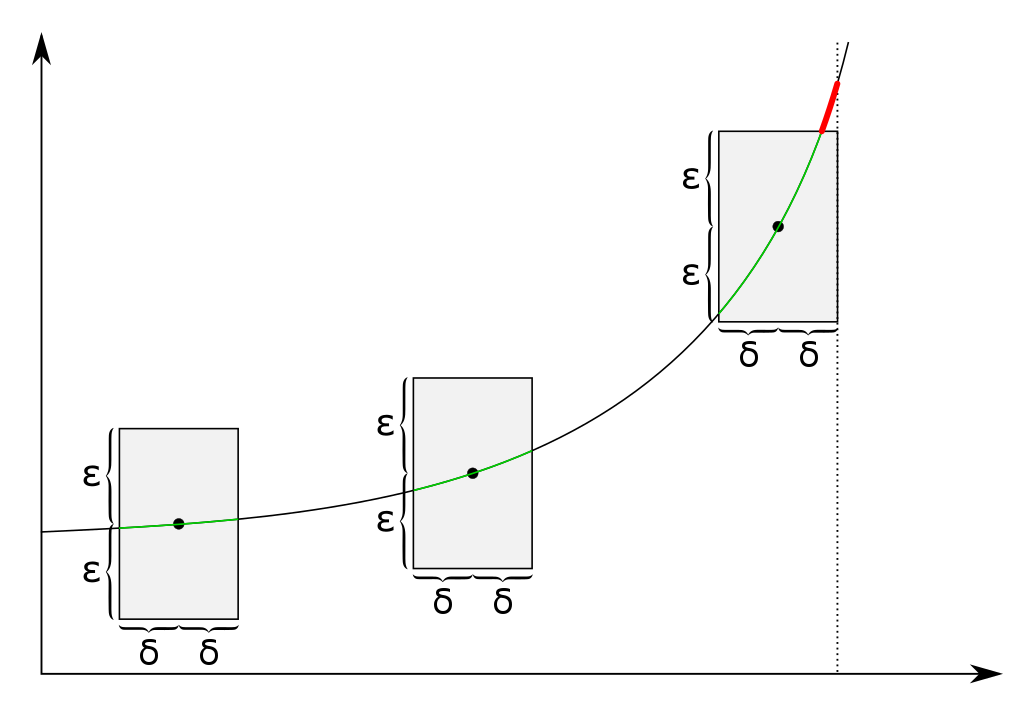
\includegraphics[width= 2.5in]{uniform_no.png} }}%
	\caption{Uniform Continuity}%
\end{figure}
\paragraph{If your function happens to satisfy $ 0<|f'(x)|<M $ for every x, then something like $\delta=\epsilon/ M$  will probably work to show uniform continuity.}
\begin{theorem}{}
	If f is continuous on a closed interval $[a, b]$, then f is uniformly
	continuous on $[a, b]$.
\end{theorem}
\begin{theorem}{}
	If $f$ is uniformly continuous on a set S and $(s_n)$ is a Cauchy sequence
	in S, then $(f(s_n))$ is a Cauchy sequence.
\end{theorem}
\begin{problem}
	Prove that if $f$ is uniformly continuous on a bounded set S,
	then $f$ is a bounded function on S.
\end{problem}
\begin{proof}
	Since, uniformly continuous functions are cauchy on a closed interval (and if the interval is not closed then we can close it! We have that power.; and cauchy sequences are bounded.
\end{proof}
\begin{definition}{}
	Let f be a function defined domain of f. Another function \~{f} is called an extension of f if. 
	\[ 
	\left\{\begin{array}{lr}
	\mathrm{dom(f) = dom(\tilde{f})} \\
	\quad\ \text{f(x) = \~{f}(x)}
	\end{array}\right\}  \forall x \in \text{dom(f)}
	\]
	Let f be defined on $(a,b)$, if f is uniformly continuous. Then,  f can be extended to \~{f} on $[a,b]$.
	
\end{definition}
\begin{theorem}{}
	A real-valued function $f$ on $(a, b)$ is uniformly continuous on $(a, b)$
	if and only if it can be extended to a continuous function $\tilde{f}$ on $[a, b]$.
\end{theorem}
\begin{theorem}{}
	Let $f$ be a continuous function on an interval $I$ [$I$ may be bounded
	or unbounded ]. Let $I^o$ be the interval obtained by removing from $I$
	any endpoints that happen to be in $I$. If f is differentiable on $I^o$ and
	if $f'$ is bounded on $I^o$, then $f$ is uniformly continuous on $I$.
\end{theorem}
\paragraph{}
\begin{problem}
	\begin{enumerate}
		\item Let f be a continuous real-valued function with domain $(a, b)$.
		Show that if $f(r) = 0$ for each rational number r in $(a, b)$, then
		$f(x) = 0$ for all $x \in (a, b)$
		\item 
		Let f and g be continuous real-valued functions on $(a, b)$ such
		that $f(r) = g(r)$ for each rational number r in $(a, b)$. Prove
		$f(x) = g(x)$ for all $x \in (a, b)$
	\end{enumerate}
	
\end{problem}
\begin{proof}
	\begin{enumerate}
		\item 
		Suppose, towards a contradiction, that there is an $x \in [a,b]$ with . As f is continuous, there is for every $\epsilon = |f(x)|/2$ some $\delta>0$ such that for all $x' \in [a,b]$    with $|x' - x| <\delta$ it follows that $|f(x) - f(x')|<\epsilon$. As , there is however a rational $x' \in [a,b]$  with $|x - x'|<\delta$ . But now   $|f(x) - \underbrace{f(x')}_{0}| < |f(x)| < |f(x)|/2 $ . Contradiction!
		
		\begin{center}
			\textbf{Or}	\end{center}
	\end{enumerate}
	Let $x\in[a,b]$, and let ${q_n}$ be a sequence of rational numbers, such that $q_n\to x$. By continuity of f, we have:
	
	$$  
	f(x) = f(\lim_{n \to \infty} q_n) = \lim_{n \to \infty} f(q_n) = 0
	$$
	
	\item
	Using the above result we can define a function $f(x) - g(x)$, and $f(x) = g(x)$ or $f(x) - g(x) = 0$   for all rationals.
	
\end{proof}

\begin{problem} Let 
	$$
	f(x) = \begin{cases} 
	0;\ \text{for x irratonal} \\
	{1 \over q};\ \text{for}\ x = {p \over q }  \\
	1,\ \text{for}\ x=0
	\end{cases}
	$$
	Show f is
	continuous at each point of $\mathbb{R \sim Q}$ and discontinuous at each point
	of $\mathbb{Q}$.	
\end{problem}

\begin{proof}
	It's easy to proof for x $\in \mathbb{Q}$. Take a sequence $(x_n)$ of irrationals such that $x_n \to p/q$. But, $f(x_n) = 0 \not = f(p/q) = 1/q$. Also, observe that the function is periodic with period 1, i.e. $f(x) = f(x+1)$.
	
	For x in set of irrational numbers. For a sequence of irrationals it's obvious that the difference b/w the function values will be 0 always.
	For a sequence of rationals we can think  of any sequence of rationals coverging to x, then the denominator value will approach infinity(it's not a formal proof). An example is shown below shown in the footnote below.
\end{proof}

\begin{problem} Let 
	$$
	f(x) = \begin{cases} 
	0;\ \text{for x irratonal} \\
	1;\ \text{for}\ x\ {rational }  \\
	\end{cases}
	$$
	Show f is
	discontinuous at each point of $\mathbb{R}$.
\end{problem}
\begin{proof}
	We begin by considering a sequence of irrational numbers $x_n$ converging to a rational $x_0$. $x_n = x_0 + {\lambda \over n}$ where $\lambda \in \mathbb{R \sim Q}$.Since, every element of $x_n$ is irrational implies $f(x_n) = 0 \not= f(x_0) = 1$. So, there exist a sequence in the domain such that $x_n \to x_0$ but $ f(x_n) \not\to  f(x_0)$ for rational $x_0$ 
	
	Similarly, using the density property of rational numbers   \footnote[1]{you need a sequence of rationals converging to the irrational x. In theory, we already know one: consider the decimal expansion of x. When x is irrational, the sequence is necessarily infinite, doesn't eventually repeat itself forever. Suppose
		$$x=m+0.d_1 d_2\ldots$$
		where m is an integer. Let
		$x_n=m+0.d_1\ldots d_n$
		In other words, $x_n$ is the decimal representation of x cut off at the n\textsubscript{th} digit after the decimal point $(x_0=m)$. Then every $x_n$ is rational, and:
		
		$$\lim_{n \to \infty}x_n=x$$ }there exist a sequence of rational numbers $(x_n)$ in $\mathbb{R}$  such that $x_n \to x_0$  for $x_0$ irrational.But $f(x_n) = 1 \not=  f(x_0) = 0$. Hence , it is not continuous. 
\end{proof}
\begin{problem}
	Let $f$ be a continuous function on $[0,\infty)$. Prove that if $f$ is
	uniformly continuous on $[k, \infty)$ for some $k$, then $f$ is uniformly
	continuous on $[0,\infty)$.
\end{problem}
\begin{problem}     
	 Let $f$ be a continuous function on $[a, b]$. Show that the function $f^{*}$ defined as 
	 $f^{*}(x) = \sup \{f(y) : a \leq y \leq x\}$, for $x \in [a, b]$, is an increasing
	 continuous function on $[a, b]$. 
\end{problem}
\begin{proof}
	Take $x_2 > x_1$ . Let $S_1 = [a,x_1]\quad\&\ S_2 = [a,x_2]$. Observe $S_1 \subset S_2$.By definition $f^{*}(x_1) = \sup \{f(y) : a \leq y \leq x_1\} $ \& $f^{*}(x_2) = \sup \{f(y) : a \leq y \leq x_2\}$. So, $f(x_1) \geq f(x) \forall x \in S_1$ and $f(x_2) \geq f(x) \forall x \in S_2$. Since, $S_1 \subset S_2$ so, $x_1 \in S_2$ implies $f(x_2) \geq f(x_1)$.
\end{proof}
%%%%% Problems%%%%%%%
%%%%%%%%%%
%%%%%%%%%%%%%%%%%%%

\section{Limits of Functions}
\paragraph*{In this section we'll formalize the notion of limit of a function and this will help us for a careful study of derivatives}
\begin{definition}{}
	Let $S \subseteq \mathbb{R}\ \text{and }\ S \not = \varnothing$, let a be a real number or symbol $ - \infty$ or $\infty$ that is a limit of a sequence in S. And let L be a real number or symbol  $ - \infty$ or $\infty$. We write $\lim_{x \to a} f(x) = L$ if:
	
	$$ \mathrm{f\ is\ a\ function\ defined\ on\ S}$$
	
	and 
	
	$$ \mathrm{for\ every\ sequence\ (x_n)\ in\ S\ converging\ to\ a,\ we\ have }\ \lim_{n \to \infty} f(x_n) = L$$
	
	The expression ``$\lim_{x \to a^S} f(x)$" is read as ``limit, as x tends to a along S,of f(x),"
	
	
\end{definition}
\paragraph{Notations} 
$$ S = (-\infty,b): 
\lim_{x \to  a} f(x) = \lim_{x \to  a^{ - }} f(x)$$
and
$$ S = (a,\infty): \lim_{x \to  a} f(x) = \lim_{x \to  a^{ + }} f(x)$$

\paragraph{Question:} Let a be a real number \& $S = (a,b) \subseteq \mathbb{R}$. Does $\lim_{x \to a^S} f(x)$ depends on S. If we take a different set $T = (a,b_1)\subseteq \mathbb{R}$ then what's the relation b/w 
$ \lim_{x \to a^S} f(x)  \&  \lim_{x \to a^T} f(x)$
\paragraph{Answer:} Since, as the $t_n \in T$ converge to a, then after some iterations the elements of sequence $t_n$ will be the elements of set S (Assuming $ S \subseteq T$).then:

$$ \lim_{x \to a^S} f(x)  = \lim_{x \to a^T} f(x)$$

\begin{theorem}{}
	Let f be a function for which the limit $L = \lim_{x\to a^S} f(x)$ exists and
	is finite. If g is a function defined on $\{f(x) : x \in S\} \cup \{L\}$ that is
	continuous at L, then $\lim_{x\to a^S} g\circ f (x)$ exists and equals g(L).
\end{theorem}
\begin{theorem}{}
	Let f be a function defined on a subset S of R, let a be a real number
	that is the limit of some sequence in S, and let L be a real number.
	then $\lim_{x \to a^S} f(x) = L$ if and only if
	\begin{equation*}
	\text{for each}\ \epsilon>0\ \text{there exists}\ \delta> 0\ \text{such that}\ 
	\end{equation*}
	\begin{equation}
	x\in S\ \text{and}\ |x - a| < \delta \Rightarrow |f(x) - L| < \epsilon.
	\end{equation}
\end{theorem}
\begin{proof}
	Assuming the statement and proving (3) is trivial so I leave it.
	
	Let $\lim_{n \to \in \infty } f(x_n) = L$:
	
	
	Now assume $\lim_{n \to  \infty} x_n = a$, but (3) fails. So, there exist a $\epsilon>0$ such that for all $\delta >0$ $|f(x_n) - f(a) |\geq \epsilon$. Take $\delta = 1/n$.So, it implies for all  $n\in \mathbb{N}$  there exist $x_n$ in S such that $|x_n - a| < 1/n$ while $|f(x_n) - f(x_0) |\geq \epsilon$. Hence aur assumption was wrong and there exist a sequence $(x_n)$ which converges to a , but $f(x_n)$ doesn't converge to $f(a)$
\end{proof}

\begin{corollary}{}
	Let f be a function defined on $J \backslash \{a\}$ for some open interval $J$
	containing a, and let L be a real number. Then $\lim_{x \to a} f(x) = L$ iff:
	
	\begin{center}
		for each $\epsilon > 0$ there exists $\delta> 0$ such that \\
		$|x - a| < \delta$ implies $|f(x) - L| < \epsilon$.
	\end{center}
\end{corollary}
\chapter{Sequence and Series of Functions}
\section{Power Series}
\begin{definition}[Power Series]{}
	$\sum_{0}^{\infty} a_n x^n$ is called a Power Series.
\end{definition}
\begin{definition}[Radius of Convergence]{def:radius-of-convergence}
	Let $\beta = \limsup |a_n|^{1 \over n}$.Then \textbf{Radius of convergence} is defined as:
	$$ R = {1 \over \beta}$$ 
\end{definition}
%\begin{problem}
%	$\sum_{0}^{\infty} a_n x^n$ converges for what value of x.
%\end{problem}
\begin{theorem}{}
	\begin{enumerate}
		\item 
		$\sum_{0}^{\infty} a_n x^n$ converges for $|x| < R$.
		\item 
		$\sum_{0}^{\infty} a_n x^n$ diverges for $|x| >R$.
	\end{enumerate}
\end{theorem}
\begin{proof}
	Take $t \in \mathbb{R}$. Take $r_t = \limsup |a_n t^n|^{1 \over n}$.Then 
	
	$$
	r_t = \limsup |a_n t^n|^{1 \over n} = |t| \limsup|a_n|^{1 \over n}= |t|\beta
	$$
	
	\paragraph{Case 1.} Let $0<R<\infty$
	
	\begin{equation*}
	r_t = \beta t = {|t| \over R} = 
	\begin{cases}|t| < R \Rightarrow \overbrace{r_t < 1}^{\text{converges by root test }}\\
	|t| > R \Rightarrow \underbrace{r_t > 1}_{\text{diverges by root test }}
	\end{cases}
	\end{equation*}
	\paragraph{Case 2.} Let $R = \infty$
	
	Here $\beta = 0$ implies $r_t = 0 <1$.So, converges for all x by root test.
	
	\paragraph{Case 3.} Let $R<0$
	
	$\Rightarrow \beta = \infty$ implies $r_t = \infty$ ; for all $|t| \not = 0$.
	Therefore Diverges.
\end{proof}
\paragraph*{Example:}
$\sum x^n$ . Here $a_n =1$.
$$
\therefore \lim \abs{a_{n+1} \over a_n} = 1 \quad \therefore \beta = 1, R = 1$$.
Therefore the series converges for $|x| < 1$. A strict inequality!.

\paragraph{Example:}
Consider the series

$$ \sum_{n=1}^{\infty} \frac{(-1)^{n+1}}{n}(x-1)^n$$

The radius of convergence for the series $ \sum_{n=1}^{\infty} \frac{(-1)^{n+1}}{n}(y)^n$ is $R = 1$, so it converges for $|y|<1$ or $ x \in (0,2)$ at $x = 0$ and $y = -1$, we have

$$ \sum_{n=1}^{\infty} \frac{(-1)^{n+1}}{n}(-1)^n = - \sum {1 \over n}$$

therefore it diverges to $- \infty$.
at x = 2

$$ \sum_{n=1}^{\infty} \frac{(-1)^{n+1}}{n}(1)^n = \sum \frac{(-1)^{n+1}}{n} = - \ln2$$


Hence,it converges \& the 
interval of convergence is $(0,2]$.
\begin{problem}
	Consider a power series $\sum a_n x_n$ with radius of convergence R.Prove that if all the coefficients an are integers and if infinitely
	many of them are nonzero, then $R \leq 1$.
\end{problem}
\begin{proof}
Given $|a_n| \geq 1$ ($\because a_n$ are integers). So, $s_n = \sup \{|a_k|: k \geq n\} \geq 1$. Further $|s_n|^{1 \over n} \geq 1$ implies $\lim |s_n|^{1 \over n} \geq 1$. Or $R \leq 1$ using \ref{def:radius-of-convergence}.
\end{proof}
\begin{problem}
Prove that if $\limsup |a_n| > 0$, then $\limsup |a_n|^{1\over n} \geq 1$.
\end{problem}
\begin{proof}
	Let $\limsup |a_n| > 0$ (notice the strict inequality!). But for sake of contradiction assume $\limsup |a_n|^{1\over n} < 1$. Then $\sum a_n$ converges, which implies $\lim a_n = 0$ (See \ref{cor:lim0}). A contradiction!
\end{proof}
\section{Uniform Convergence}

\begin{definition}[Pointwise Convergence]{}
	Let $(f_n)$ be a sequence of real-valued functions defined on a set $S \subseteq \mathbb{R}$. The sequence $(f_n)$ converges pointwise [i.e., at each point] to a
	function $f$ defined on S if
	
	$$ \lim\limits_{n\to \infty} f_n (x) = f(x) \quad \text{for all} \quad x\in S$$
	We often write $\lim f_n = f$ pointwise $[on\ S]$ or $f_n \to f$ pointwise [on S].
	
	
	Now observe $f_n\to f$ pointwise on S means exactly the following:
	
	for each $\epsilon>0$ and x in S there exists N such that
	$$ |f_n(x) - f(x)| < \epsilon\quad \text{for}\quad n>N$$
	
	Note the value of N depends on both $\epsilon$ and x in S. 
\end{definition}
\paragraph{Example}
Let $f_n(x) = x^n$ for $x\in [0, 1]$. Then $f_n\to f$ pointwise on $[0, 1]$ where
$f(x) = 0$ for $x\in [0, 1)$ and $f(1) = 1$. Or we can write:

$$ \lim_{n \to  \infty}   f_n(x) = \lim_{n \to \infty} x^n = \begin{cases}
1\quad \text{if} \ x = 1\\
0 \quad \text{else}
\end{cases}            $$
Consider, 
$$  f(x)  = \begin{cases}
1\quad \text{if} \ x = 1\\
0 \quad \text{else}
\end{cases}            $$
Then we can write $\lim_{n \to \infty} f_n (x) = f(x)$.
\paragraph{}
\begin{definition}[Uniform Convergence]{}
	Let $(f_n)$ be a sequence of real-valued functions defined on a set
	$S\subseteq \mathbb{R}$. The sequence $(f_n)$ converges uniformly on S to a function $f$ defined on S if
	
	for each $\epsilon>0$ there exists a number N such that 
	
	$$ |f_n(x) - f(x)| < \epsilon\quad \text{for all}\quad x \in S \quad and \quad n>N$$.
	We write $\lim f_n = f$ uniformly on S or $f_n \to f$ uiniformly on S.
\end{definition}


\paragraph{Example:}Define,

$$f_n(x) = x^n\quad for\quad x\in [0,1]$$

$$ f(x) = \begin{cases}
0, x\not = 0 \\
1, x = 0
\end{cases}$$

then $\epsilon = 1/2$,then we consider for all $x \in [0,1]$ and all $n >N$.

$$ |f_n(x) - f(x)| < \epsilon = 1/2$$

$|x| \leq 1$ \& $n>N$

$$\Rightarrow |f_n - f| < 1/2$$
at $x = 0$ it's not possible as $|0 - 1| < 1/2$ is not true. So, not uniformly converging.

\paragraph{Example}


Let $f(x) = {1 \over n} sin(nx)$ $\forall x \in \mathbb{R}$

for any x $\lim_{n \to  \infty} f_n(x) = 0$ pointwise on R. Define $f(x) = 0$ then $f_n \to f$. In fact $f_n \to f$ uniformly on R. Also, let $N = 1/\epsilon$ .Then for $n>N$ and all $x \in \mathbb{R}$ we have

$$ |f_n(x) - f(x)| = |f_n(x) - 0| = \abs{{1 \over n}sin(nx)} \leq {1 \over n} <{1 \over N} = \epsilon$$
Since, N is independent of x.

\paragraph{}

\begin{theorem}{}
	Uniform limit of continuous function is continuous.More precisely, let $(f_n)$ be a sequence of functions on a set $S\subseteq \mathbb{R}$, suppose $f_n\to f$ uniformly on S, and suppose $S = dom(f)$. If each $f_n$ is
	continuous at $x_0$ in S, then f is continuous at $x_0$. [So if each $f_n$ is continuous on S, then f is continuous on S.]
\end{theorem}
%%%%%%%%%%%%%%%%%%%%%%%%%%%%%%%%%%%%%%
%%%%%%%%%%%%%%%%%%%%%%%%%%%%%%%%%%%%%%
%%%%%%%%%%%%%%%%%%%%%%%%%%%%%%%%%%%%%%
%%%%%%%%      proof left     %%%%%%%%%%%%%%\\
%%%%%%%%%%%%%%%%%%%%%%%%%%%%%%%%%%%%%%
%%%%%%%%%%%%%%%%%%%%%%%%%%%%%%%%%%%%%%
%%%%%%%%%%%%%%%%%%%%%%%%%%%%%%%%%%%%%%
\paragraph{Remark} Remember $f_n \to f$ on S uniformly iff,

$$ \limsup \limits_{n \to \infty} \{|f_n(x) - f(x)|: x \in S\} = 0$$
\paragraph{}

We can also consider $\sum_{k = 0}^{\infty} g_k(x)$, where $g_k$ is a function of $S\subset\mathbb{R}$.
\begin{theorem}{}
	If $g_k$ is continuous $\forall k$ and if $\sum g_k$ converges uniformly, then it converges to a continuous function on S.
\end{theorem}

\begin{proof}
	Let $f_n = \sum_{k = 0}^{n} g_k(x)$ is continuous on S and $f_n(x) = \sum_{k = 0}^{\infty} g_k(x)$ uniformly.
	
	$\therefore f(x) = \sum_{k = 0}^{\infty} g_k(x)$ is continuous.
\end{proof}

\begin{corollary}{}
	$f(x) = \sum a_n x^n $ is a continuous function if the convergence is uniform.
\end{corollary}
\begin{problem}
	Prove that if $(f_n)$ is a sequence of uniformly continuous functions
	on an interval $(a, b)$, and if $f_n\to f$ uniformly on $(a, b)$, then $f$ is
	also uniformly continuous on $(a, b)$.
\end{problem}
\begin{proof}
	We need to show that $\forall \delta>0\ \exists \epsilon>0$ such that $|x-y|<\delta$ implies $|f(x)-f(y)|<\epsilon.$
	
Using triangualar inequality we can show that:
$$|f(x)-f(y)| \leq |f(x)-f_n (x)|+|f_n(x)-f_n(y)|+|f_n (y)-f(y)|$$ 
Using the $\epsilon/3$ argument we can show that, there exists a $N$ such that $n>N_1$ implies $ |f_n(x)-f_n(y)| <\epsilon/3$ (it's uniform cont.) and $|x-y| < \delta$.And we can apply definition of uniform convergence to show $|f_n (y)-f(y)| < \epsilon/3$ by choosing some $N_2$ for x and then some $N_2$ for y.So we have for $n> N = max(N_1,N_2,N_3)$. 
$$|f(x)-f(y)| < 3\cdot {\epsilon \over 3}= \epsilon$$

\end{proof}


\chapter{Differentiation}
\section{Why differentiation? \\ Better ask Newton.}
\begin{definition}{}
	$f$ is a real-valued function on an open interval $I$ Let $a \in I$. Then $f$ is differentiable at ``a" if the limit :
	$$ \lim\limits_{x \to a} \frac{f(x)-f(a)}{x-a}$$
	exists \& is finite. We also sayy $f$ has a derivative at a.
	
	$$ f'(x) = \lim\limits_{x \to a} \frac{f(x)-f(a)}{x-a}$$ 
	
	\paragraph{Remark}
	'$f'(x)$ itself is a function with domain $f \subseteq dom f$.
\end{definition}
\begin{theorem}{}
If	$f$ be diff. at $x = a$. Then $f$ is continuous at a.
\end{theorem}

\begin{proof}
	$f(x) = (x - a) \frac{f(x)-f(a)}{x-a} + f(a)$
	\begin{align}
	\therefore \lim_{x \to a}f(x) = \lim_{x \to a}(x - a) \lim_{x \to a}\frac{f(x)-f(a)}{x-a} + \lim_{x \to a}f(a) = 0\cdot f'(a) + f(a)\\
	\end{align}
\end{proof}

\begin{theorem}[Properties]{} 
	If $f, g$ are diff. at $x = a$ and $c \in \mathbb{R}$ then
	\begin{enumerate}
		\item 
		$(cf)'(a) = cf'(a)$
		\item 
		$(f+g)'(a) = f'(a)+g'(a)$
		\item 
		$(fg)'(a) = f'(a)g(a)+f(a)g'(a)$
		\item 
		$({f \over g})'(a) = \frac{f'(a)g(a) - f(a)g'(a)}{g(a)^2}$
	\end{enumerate} 
\end{theorem}


\begin{theorem}[\textbf{Chain Rule}]{}
	$f $ be differentiable at $x = a$ and $g$ be differentiable at $f(a)$. Then $(g \circ f )(x)$ is diff at x = a. And  $(g \circ f )'(x) = g'(f(x)) \cdot f'(x)$
\end{theorem}

\section{Mean Value Theorem}

\begin{theorem}{}
If $f$ is defined on an open interval containing $x_0$, if $f$ assumes its
maximum or minimum at $x_0$, and if $f$ is differentiable at $x_0$, then
$f '(x_0) = 0$.
\end{theorem}
\begin{theorem}[Rolle’s Theorem]{thm:rolles theorem}
	Let $f$ be a continuous function on $[a, b]$ that is differentiable on $(a, b)$
	and satisfies $f(a) = f(b)$. There exists [at least one] $x$ in $(a, b)$ such
	that $f '(x) = 0$.
\end{theorem}
\begin{theorem}[Mean Value Theorem]{thm:mean value}
Let $f$ be a continuous function on $[a, b]$ that is differentiable on $(a, b)$.
Then there exists [at least one] x in $(a, b)$ such that:
$$ f'(x) = \frac{f(b) - f(a)}{b - a }$$
\end{theorem}
\begin{corollary}{}
Let $f$ be a differentiable function on $(a, b)$ such that $f '(x) = 0$ for all
$x \in(a, b)$. Then $f$ is a constant function on $(a, b)$.
\end{corollary}
%%%%%%%%%%%%%%%%%%%%%%%%%%%%%%%%%%%%%%%%%%%%%%%%%%%%%%%
\begin{corollary}{}
Let $f$ and $g$ be differentiable functions on $(a, b)$ such that $f ' = g'$ on
$(a, b)$. Then there exists a constant c such that $f(x) = g(x) + c$ for
all $x \in(a, b)$.
\end{corollary}

\begin{corollary}{}
Let $f$ be a differentiable function on interval $(a,b)$, then:
\begin{enumerate}[(i.)]
\item $f$ is strictly increasing if $f '(x) > 0$ for all $x \in(a, b)$;
\item $f$ is strictly decreasing if $f '(x) < 0$ for all $x \in(a, b)$;
\item $f$ is increasing if $f '(x) \geq 0$ for all $x \in(a, b)$;
\item $f$ is decreasing if $f '(x) \leq 0$ for all $x \in(a, b)$;
\end{enumerate}
\end{corollary}

\begin{theorem}[Intermediate Value Theorem for Derivatives.]{}
	Let $f$ be a differentiable function on $(a, b)$. If $a < x_1 < x_2 < b$, and
	if c lies between $f'(x_1)$ and $f '(x_2)$, there exists [at least one] x in
	$(x_1, x_2)$ such that $f '(x) = c$.
\end{theorem}
\begin{problem}
Let $f$ be differentiable on R with $a = \sup\{|f'(x)| : x \in \mathbb{R}\} < 1$. Select $x_0 \in \mathbb{R}$ and define $x_n =f(x_{n - 1})$ for $n \geq 1$. Thus $x_1 = f (x_0 ), x_2 = f (x_1 )$, etc. Prove $(x_n )$ is a convergent sequence.
\end{problem}
\begin{proof}
	Using the mean value theorem we can see $f$ is a contraction, because
	
	$$|f(x) - f(y)| = |f'(c)||x-y| \leq a|x-y|$$
	With $a < 1$.
	
	
	Now to see it is a convergent / cauchy sequence, select $x_0$ and note $x_n = f(x_{n-1})$, what can you say of $$|x_n - x_m|$$ for arbitrary $m, n$?
	
	HINT: Use triangle inequality and $|x_n - x_{n+1}| \leq a^n|x_0 - x_1| $ . For alternate proof refer to Problem \ref{problem-2^n}
	
 Suppose $m > n$ then:
	
	$$|x_n - x_m| \leq |x_n - x_{n+1}| + |x_{n+1} - x_{n+2}| + \dots + |x_{m-1} + x_{m}|$$
	
	$$\leq \sum_{k = n}^m a^k |x_0 - x_1| \leq \sum_{k = n}^{\infty} a^k |x_0 - x_1| < +\infty $$
	Now, because this last series converges ($a < 1$), by the Cauchy criterion, given $\varepsilon >0$, there is some $N$ such that $$\sum_{k = N}^{\infty} a^k |x_0 - x_1| < \varepsilon $$
	If we pick $n,m \geq N$ we're done, now we know $x_n$ is a Cauchy sequence in $\mathbb{R}$, and thus has a limit $x$, now $$x = \lim x_n = \lim f(x_{n-1}) = f(\lim x_{n-1}) = f(x)$$ hence $x$ is a fixed point. To see its uniquenes suppose $x_1, x_2$ are two fixed points, then:
	
	$$|x_1 - x_2| = |f(x_1) - f(x_2)| \leq a|x_1 - x_2|   $$
	
	With $a < 1$ this is only true if $x_1 = x_2$.
\end{proof}

\section{Taylor Theorem}
\begin{definition}[Taylors Series]{def:taylor}
Let $f$ be a function defined on some open interval containing c. If $f^k (c)$
exists $\forall k$, then the series:
$$   \sum_{k=0}^{\infty} \frac{f^{(k)} (c)}{k!} (x -c)^k        $$
is called as \textbf{Taylor Series} of function $f(x)$ about c. For $n \geq 1$; remainder $R_n (x)$ is defined as:
$$R_n (x) = f(x) - \sum_{k=0}^{n-1} \frac{f^{(k)} (c)}{k!} (x -c)^k  $$
The remainder is important because, for any x;
$$  f(x) =   \sum_{k=0}^{\infty} \frac{f^{(k)} (c)}{k!} (x -c)^k \quad \text{if and only if}\quad \lim\limits_{n \to \infty} R_n(x) = 0 $$
\end{definition}
\begin{theorem}{thm:taylor}
Let $f$ be defined on $(a, b)$ where $a < c < b;$ here we allow $a = - \infty$
or $b = \infty$. Suppose the $n\textsuperscript{th}$ derivative $f ^{n}$ exists on $(a, b)$. Then for
each $x \not = c$ in $(a, b)$ there is some $y$ between $c$ and $x$ such that
$$ R_n (x) = \frac{f^n (y)}{n!}(x-c)^n$$
\end{theorem}
\begin{corollary}{}
	Let $f$ be defined on interval $(a,b)$ and $a<c<b$. If $f^k$ exists $ \forall k$ , \& there exists a single constant $C$ such that $\abs{f^k (c)} \leq C$, then 
	$$ \lim_{n \to \infty} R_n (x) = 0 \quad \forall\ x \in (a,b) $$
\end{corollary}

\chapter{Die Theorie der Integration}
\section{Integrals}

\begin{definition}[The Darboux Integral]{def:darboux sum}
Let $f$ be a bounded function on a closed interval $[a, b]$.1 For $S \subseteq[a, b]$,
we adopt the notation:
\begin{itemize}
	\item 
	$M(f, S) = \sup\{f(x) : x \in S\}$
	\item 
	$m(f, S) = \inf\{f(x) : x \in S\}$.
\end{itemize}
A partition of $[a, b]$ is any finite ordered subset $P$ having the form
$$P = \{a = t_0 < t_1 < \cdots< t_n = b\}.$$
	The upper Darboux sum $U(f, P)$ of $f$ with respect to $P$ is the sum:
	$$U(f,P) = \sum \overbrace{M(f, [t_{k - 1}, t_k])\cdot (t_k - t_{k- 1})}^{\text{Area of rect. above the curve} }$$
	
	and the lower Darboux sum $L(f, P)$ is:
		$$L(f,P) = \sum \underbrace{m(f, [t_{k- 1}, t_k])\cdot (t_k - t_{k- 1})}_{\text{Area of rect. below the curve}}$$
		Note
		$$U(f,P) \leq M(f,[a,b])(b-a); $$
		and 
		$$ L(f,P) \geq m(f,[a,b])(b-a) ; $$
		
		The upper Darboux integral $U(f)$ of $f$ over $[a,b]$ is defined by
		$$ U(f) =  \inf \{U(f,P):P\ \text{is a partition of }[a,b]\}$$
		and the lower Darboux integral is
		$$L(f) = \sup\{L(f,P):P\ \text{is a partition of }[a,b]\}$$
		We say $f(x)$ is integrable if on $[a,b]$ if $L(f)=U(f)$.
\end{definition}
\paragraph{Observe:}

$L(f,\{a,b\})\leq L(f,P) \leq U(f,P)\leq U(f,\{a,b\})$. 


\begin{lemma}{}
	Let $f$ be a bounded function on $[a, b]$. If $P$ and $ Q$ are partitions of
	$[a, b]$ and $ P \subseteq Q$, then
	$$L(f,P)\leq L(f,Q)\leq U(f,Q)\leq U(f,P)$$
\end{lemma}
 \begin{lemma}{}
 	If $f$ is a bounded function on $[a, b]$, and if $P$ and $Q$ are partitions of
 	$[a, b]$, then $L(f, P) \leq U(f, Q)$
 \end{lemma}

\begin{lemma}{}
If $f$ is a bounded function on $[a, b]$, then $L(f) \leq U(f)$.
\end{lemma}
\begin{theorem}{}
	A bounded function $f$ on $[a, b]$ is integrable if and only if for each
	$\epsilon > 0$ there exists a partition P of $[a, b]$ such that
	$$U(f,P)-L(f,P) < \epsilon$$
\end{theorem}

\begin{definition}[Mesh]{}
	The $mesh$ of a partition P is the maximum length of the subintervals
	comprising P. Thus if:
	$$P = \{a = t_0 < t_1 <t_2 \cdots <t_n=b\},$$
	then 
	$$ \text{mesh}(P) = \max \{t_k - t_{k-1}: k = 1,2,3,\ldots,n\}$$
\end{definition}

\begin{definition}[Rienmann Sum \nocite{wiki:integral}]{}
	Let ${f:[a,b]\rightarrow \mathbb {R} }$ be a function defined on a closed interval $[a,b]$ of the real numbers, $\mathbb {R}$ , and
	$$P = \{a = t_0< t_1< t_2 \cdots t_n = b\}$$
	be a partition of $[a,b]$. A riemann sum of $f$ associated with  the  partition P is a sum of the form
	$$\sum_{k = 1}^{n} f(x_k)(t_k - t_{k-1})$$
	where $x_k \in [t_{k-1},t_k]$ for $k = 1,2, 3, \ldots n$. The choice of $x_k$ is arbitrary, so there are infinitely many Riemann sums associated with a single function and partition.
\end{definition}

\begin{definition}[Riemann Integral]{}
The function $f$ is Riemann integrable on $[a, b]$ if there exists a
number $r$ such that for each $\epsilon > 0$ there exists
$\delta > 0$ such that
$$|S-r| < \delta $$
	for every Rienmann sum of $f$ associated with the partition P having mesh$(P)< \delta$. The number $r$ is the Riemann integral of $f$ on $[a,b]$ and will be provisionally written as $\mathcal{R} \int_{a}^{b}f$.
\end{definition}

\begin{theorem}{}
	A bounded function $f$ on $[a, b]$ is integrable if and only if for each
	$\epsilon > 0$ there exists a $\delta > 0$ such that
	$mesh(P) < \delta$ implies
	$$U(f, P) - L(f, P) < \epsilon$$
	
	for all partitions P of $[a, b]$.
\end{theorem}

%%%%%%%%%%%%%%%%%%%%%%%%%%%%%%%%%%%%%%%%%
%%%%%%%%%%%%%%%%%%%%%%%%%%%%%%%%%%%%%%%%%
%%%%%%%%%%%%%%%%%%%%%%%%%%%%%%%%%%%%%%%%%\\
%%%%%%%%%%%%%%%%%%%%%%%%%%%%%%%%%%%%%%%%%\\
%%%%%%%%%%%%%%%%%%%%%%%%%%%%%%%%%%%%%%%%%\\


\subsection{Fundamental Theorem of Calculus}

\begin{theorem}{thm:fund-cal-1}
If $g$ is a continuous function on $[a, b]$ that is differentiable on $(a, b)$,
and if $g'$ is integrable on $[a, b]$, then
$$\int_{a}^{b} g' = g(b) - g(a)$$
\end{theorem}
\begin{theorem}{thm:fund-cal-2}
	Let $f$ be an integrable function on $[a, b]$. For $x$ in [a, b], let
	$$F(x) = \int_{a}^{x}f(t)dt.$$
	Then $F$ is continuous on $[a, b]$. If f is continuous at $x_0$ in $(a, b)$, then
	$F $ is differentiable at $x_0$ and
	$$F'(x) = f(x)$$
\end{theorem}


\subsection{Intermediate Value Theorem for Integrals.}

\begin{theorem}[Intermediate Value Theorem for Integrals.]{}
	If $f$ is a continuous function on $[a, b]$, then for at least one $x$ in $(a, b)$
	we have:
	\[  f(x) = \int_{a}^{b} f   \]
\end{theorem}


\begin{problem}
	Let $f(x) = x$ for rational $x$ and $f(x) = 0$ for irrational $x$.
	\begin{enumerate}
		\item
		Calculate the upper and lower Darboux integrals for $f$ on the
		interval $[0, b]$.
		\item 
		Is $f$ integrable on $[0, b]$?
	\end{enumerate}
\end{problem}
\chapter{Differentiation and Integration of Power Series}
\begin{theorem}[Weierstrass M-test]{}
	Let $(M_k)$ be a sequence of non-negative real numbers where $\sum M_k < \infty$. If $|g_k(x)| \leq M_k$ for all $x$ in a set $S$, then $\sum g_k$ converges
	uniformly on S
\end{theorem}
\begin{proof}
	Let $\epsilon>0$ , $\exists N $ such that $n \geq m > N \Rightarrow \sum_{k = m}^{\infty} M_k < \epsilon$. Then if $ n \geq m > N $ and $  x \in S $,
	$$\abs{\sum_{k = m}^{n}g_k(x)} \leq\sum_{k = m}^{n}|g_k(x)| \leq \sum_{k = m}^{n}M_k < \epsilon $$
	$ \therefore $ by cauchy criterion on uniform cont. on S,
	$ \sum g_k $ converges uniformly on S.
\end{proof}
\begin{problem}
	Show that if the series $ \sum g_n $  converges uniformly on a set S, then
	$$\lim\limits_{n \to \infty} \sup\{|g_n(x)|: x\in S\} = 0 $$
\end{problem}
\begin{proof}
	For $\epsilon > 0$ , $\exists N$ such that $n \geq m > N \Rightarrow \left| \sum_{m}^{n} g_k (x)\right| < \epsilon$.\\
	In particular $n>N$ 
	$$\Rightarrow |g_n| < \epsilon\ \forall \ x \in S $$
	$$\therefore \sup \{|g_n(x)| : x \in S \} \leq \epsilon$$
	$$\lim_{n \to \infty }\sup \{|g_n(x)|: x\in s\} = 0$$
\end{proof}


\begin{theorem}{}
	Let $ \sum a_n x^n  $ be a power series with radius of convergence $R > 0$. If $0 < R_1 < R$, then the power series converges
	uniformly on $[-R_1, R_1]$ to a continuous function.
\end{theorem}

\begin{lemma}
	If the power series $ \sum a_n x^n  $  has radius of convergence R, then the
	power series
	$$\sum n a_n x^n \qquad \& \qquad \sum \dfrac{a_n}{n+1} x^{n+1}$$
	have the same radius of convergence R.
\end{lemma}

\begin{theorem}{}
	Suppose $f(x) =  \sum a_n x^n  $ has radius of convergence $R > 0$ Then
	$$\int_{0}^{x}f(t) dt = \sum \frac{a_n}{n+1}x^{n+1}\ \ \forall x < R$$
\end{theorem}

\begin{theorem}{}
	Let $f(x) =  \sum a_n x^n  $ have radius of convergence $R > 0$. Then $f$ is
	differentiable on $(-R, R)$ and
	$$f'(x) = \sum_{n=1}^{\infty} a a_n x^{n-1}\quad \forall |x| < R$$
\end{theorem}
\begin{theorem}[Abel's Theorem]{}
	Let $f(x) =  \sum a_n x^n  $ be a power series with $0<  R<\infty$. If the series converges at $x = R$, then $f$ is continuous
	at $x = R$. If the series converges at $x = -R$, then $f$ is continuous
	at $x = -R$.
\end{theorem}



\appendix
\addappheadtotoc
\chapter{Power series of some common functions} 

\begin{description}
\item [\textbf{Exponential Series}]
$$e^{x} = \sum^{\infty}_{n=0} \frac{x^n}{n!} = 1 + x + \frac{x^2}{2!} + \frac{x^3}{3!} + \cdots.$$
It converges for all $x \in \mathbb{R}$.
\item[Natural logarithm] 
\[\begin{aligned}
\ln(1-x) &= - \sum^{\infty}_{n=1} \frac{x^n}n = -x - \frac{x^2}2 - \frac{x^3}3 - \cdots , \\
\ln(1+x) &= \sum^\infty_{n=1} (-1)^{n+1}\frac{x^n}n = x - \frac{x^2}2 + \frac{x^3}3 - \cdots .
\end{aligned}\]
They converge for $|x| < 1$
\item[Geometric series]
\[\begin{aligned}
\frac{1}{1-x} &= \sum^\infty_{n=0} x^n \\
\frac{1}{(1-x)^2} &= \sum^\infty_{n=1} nx^{n-1}\\
\frac{1}{(1-x)^3} &= \sum^\infty_{n=2} \frac{(n-1)n}{2} x^{n-2}.
\end{aligned}\] All are convergent for \(|x| < 1\). These are special cases of Binomial Series.

\item[Binomial series] The binomial series is a power series
\[(1+x)^\alpha = \sum_{n=0}^\infty \binom{\alpha}{n} x^n\]
whose coefficients are the generalized
\href{https://en.wikipedia.org/wiki/Binomial_coefficient}{binomial coefficients}
\[\binom{\alpha}{n} = \prod_{k=1}^n \frac{\alpha-k+1}k = \frac{\alpha(\alpha-1)\cdots(\alpha-n+1)}{n!}.\]
\item[Trignometric Functions]
The usual trigonometric functions and
their inverses have the following power series:

\[\begin{aligned}
\sin x &= \sum^{\infty}_{n=0} \frac{(-1)^n}{(2n+1)!} x^{2n+1} &&= x - \frac{x^3}{3!} + \frac{x^5}{5!} - \cdots && \text{for all } x\\[6pt]
\cos x &= \sum^{\infty}_{n=0} \frac{(-1)^n}{(2n)!} x^{2n} &&= 1 - \frac{x^2}{2!} + \frac{x^4}{4!} - \cdots && \text{for all } x\\[6pt]
\tan x &= \sum^{\infty}_{n=1} \frac{B_{2n} (-4)^n \left(1-4^n\right)}{(2n)!} x^{2n-1} &&= x + \frac{x^3}{3} + \frac{2 x^5}{15} + \cdots && \text{for }|x| < \frac{\pi}{2}\\[6pt]
\sec x &= \sum^{\infty}_{n=0} \frac{(-1)^n E_{2n}}{(2n)!} x^{2n} &&=1+\frac{x^2}{2}+\frac{5x^4}{24}+\cdots && \text{for }|x| < \frac{\pi}{2}\\[6pt]
\arcsin x &= \sum^{\infty}_{n=0} \frac{(2n)!}{4^n (n!)^2 (2n+1)} x^{2n+1} &&=x+\frac{x^3}{6}+\frac{3x^5}{40}+\cdots && \text{for }|x| \le 1\\[6pt]
\arccos x &=\frac{\pi}{2}-\arcsin x\\&=\frac{\pi}{2}- \sum^{\infty}_{n=0} \frac{(2n)!}{4^n (n!)^2 (2n+1)} x^{2n+1}&&=\frac{\pi}{2}-x-\frac{x^3}{6}-\frac{3x^5}{40}-\cdots&& \text{for }|x| \le 1\\[6pt]
\arctan x &= \sum^{\infty}_{n=0} \frac{(-1)^n}{2n+1} x^{2n+1} &&=x-\frac{x^3}{3} + \frac{x^5}{5}-\cdots && \text{for }|x| \le 1,\ x\neq\pm i
\end{aligned}\]

All angles are expressed in radians.The numbers $B_k$
appearing in the expansions of $\tan x$ are the
\href{https://en.wikipedia.org/wiki/Bernoulli_number}{Bernoulli numbers}. The $E_k$ in the expansion  of $\sec x$ are
\href{https://en.wikipedia.org/wiki/Euler_number}{Euler numbers}. 
\end{description}



\bibliographystyle{unsrt}
\bibliography{ref}


\end{document}
